\documentclass[12pt,a4paper]{report}
\usepackage{a4-mancs}
\usepackage{pslatex}
\usepackage{lastpage}
\usepackage{fancyhdr}
\usepackage{graphicx}
\usepackage{listings}
\usepackage{amsmath}
\usepackage{algorithm}
\usepackage{algorithmic}
\usepackage{calc}
\usepackage[greek,english]{babel}
\usepackage[toc,page]{appendix}
\usepackage[nottoc]{tocbibind}
\usepackage{amsfonts}
\usepackage{url}
\usepackage{datetime}
\DeclareGraphicsExtensions{.png}
\pagestyle{fancyplain}

\newcommand{\HRule}{\rule{\linewidth}{0.5mm}}
\begin{document}
\begin{titlepage}
\begin{center}

\includegraphics[width=0.15\textwidth]{logo.png}~\\[1cm]

\textsc{\LARGE University of Manchester}\\[1.5cm]

\textsc{\Large School of Computer Science}\\[0.5cm]

\textsc{\Large Third Year Project}\\[0.5cm]
% Title
\HRule \\[0.4cm]
{ \huge \bfseries Alan Turing's morphogenesis: on the wonders of nature}\\[0.4cm]

\HRule \\[1.5cm]


\begin{minipage}{0.4\textwidth}
\begin{flushleft} \large
\emph{Author:}\\
Vasilis \textsc{Nicolaou}
\end{flushleft}
\end{minipage}
\begin{minipage}{0.4\textwidth}
\begin{flushright}
{\large \emph{Degree Programme:}} \\MEng(Hons) Software Engineering
\end{flushright}
\end{minipage}
$$$$
$$$$
$$$$
\begin{center}
\emph{Supervisor:} \\
Dr.~Eva M. \textsc{Navarro-Lopez}
\end{center}
% Bottom of the page

\newdateformat{mydate}{\monthname[\THEMONTH] \THEYEAR}
\vfill
{\mydate{\today}}

\end{center}
\end{titlepage}

\pagenumbering{roman}
\begin{abstract}
Alan Turing in 1952 described mathematically how cells can self-organise to form a variety of structures. He called this phenomenon ‘morphogenesis’, which means the creation of shape. Cells communicate with each other by diffusion, a process where chemical compounds or morphogens move from higher to lower concentrations. The project studies various aspects of morphogenesis and analyses several reaction-diffusion mathematical models. The main goal was to translate the simulations of such dynamical systems into descriptive animations of the processes involved. The project exploits morphogenesis exploring the phenomenon of cell mutation. Producing sound from reaction-diffusion mathematical models is also introduced. Finally, the project proposes applications of morphogenesis in engineering achieving the merging of the separate worlds of biology, mathematics, computer science, engineering and arts.
\paragraph{Title of project:}
Alan Turing's morphogenesis: on the wonders of nature.
\paragraph{Author:}

Vasilis Nicolaou
\paragraph{Supervisor:}
Eva M. Navarro Lopez

\vfill
\newdateformat{mydate}{\monthname[\THEMONTH] \THEYEAR}
\begin{center}
{\mydate{\today}}
\end{center}
\end{abstract}

\renewcommand{\abstractname}{Acknowledgements}
\begin{abstract}
I would like to thank my supervisor, Dr. Eva M. Navarro Lopez, for her academic wisdom, her caring manner and her constant help throughout the year which was essential for completing this project.

I also thank my friends and co-students for the funny moments and inspirational conversations throughout a challenging and difficult year.

Last but not least, I thank my family for believing and supporting me throughout my University studies.  
   
\end{abstract}
\tableofcontents
\listoffigures
\listoftables
\listofalgorithms
\newpage
\pagenumbering{arabic}
\cfoot{\thepage\ of \pageref{LastPage}}

\chapter{Introduction}

	\section{Morphogenesis}

	Morphogenesis is the biological process that defines how a system of cells is organised and shaped. The word originates from the Greek words `\greektext morf'h\latintext ' which means shape and `\greektext g'enesic\latintext ' which means birth. Alan Turing in his paper `The chemical basis of morphogenesis' gives a mathematical model that can approximate how an embryo develops its various organs \cite{turing_chemical_1990}. 
	
    The challenge was to show how from a single cell that replicates into identical cells, various organs are developed with different functionalities. For example, in a human embryo, there is initially a single cell that was produced from half the characteristics of the mother and half of the father. Eventually, millions of cells are generated. Nevertheless, they manage to differentiate into groups that form parts of different organs. 
	
Turing defined a hypothetical chemical substance called morphogen. A morphogen is an abstract term which represents a chemical compound that gives the cell certain properties according to its concentration. A cell, therefore, may be defined as a vector of morphogens that react together forming the state of a cell. In addition, each cell has several neighbouring/adjacent cells. 

When cells with different concentrations of chemical compounds are connected, the phenomenon of diffusion is observed. The membrane of a cell has a property that allows chemical substances to move from higher to lower concentrations. This is how cells communicate. Diffusion is further explained in Section \ref{diffusion}.
	
By constructing mathematical equations that approximate chemical reactions and diffusion, one can define models that approximate the phenomenon of morphogenesis. Such models are described in Chapter \ref{morphogenesis}.

	\section{Project objectives}
	
    This project studies the idea of morphogenesis that Alan Turing proposed and subsequently produces software applications that simulate various models of the reaction-diffusion biological process. The simulations combine graphs that may be used for analysis or testing and movies\footnote{Movies are available at: \url{http://www.youtube.com/watch?v=2JppD_Mw_3k}} that show how cells are  organised forming structural patterns. Simulations also visualise the effects of cell mutations, processed as random changes in morphogen concentrations after a system develops a structured shape.

    The project goes a step further and introduces applications of morphogenesis in engineering. A process scheduling algorithm inspired by the reaction-diffusion concept has been developed and compared to traditional schedulers such as the Round Robin. The idea of how a scheduler is related to morphogenesis is not obvious and is described in section \ref{schedulers}.
	
    Some experiments study the possibility of producing sound by the use of mathematical models that produce continuous oscillations. Due time limitations, experiments are not extensive and no meaningful sound output was produced. However, readers and future researches of the subject are encouraged into further study of such experiments, since graphs present a behaviour similar to sound waves.  

	
    \section{Background}
    Morphogenesis is defined by Alan Turing as the process of how cells of an embryo create shape out of an initially chaotic behaviour \cite{turing_chemical_1990}. Cells are interacting with each other by diffusing chemical substances which in Turing's morphogenesis model are defined as morphogens. The term morphogen is abstract and should not be confused with DNA genes, chromosomes or certain chemical elements. 
A morphogen is considered to be a chemical substance that has some theoretical properties which give to cell specific characteristics. Morphogens may also react with each other in the same way chemical molecules do. Reactions and diffusion happen over time and thus morphogenesis process can be a dynamical system.   
Thus, it can be modelled mathematically using differential equations, by suggesting that each cell has a state according to its morphogen concentrations and that state is subject to change over time.

The approach followed for simulation and analysis of morphogenesis' models uses a variety of concepts of the mathematical, biochemical and programming domain. Such concepts are discussed in this report providing the knowledge basis that is necessary for the reader to follow the approach and the implementation procedure of the project.

Finally, various papers and articles \cite{garvie_methodology}\cite{heineike_modeling_2002}\cite{kassam_solving_2003} that study the phenomenon of morphogenesis and pattern generation were used to identify mathematical models of the reaction-diffusion process and were the spark for further exploration of ideas related to morphogenesis. 






	\section{Approach}

The approach was partitioned in several stages. Since the project has a strong mathematical component, background knowledge of the mathematical concepts that were involved are presented. The information on the mathematical knowledge that is required  is given by Alan Turing in his paper \cite{turing_chemical_1990}. To sum up, this subject merges ordinary differential equations, integration methods, algebra and computational theory.

Application of mathematical concepts from dynamical systems theory is required to build an understanding on how software applications of mathematical models are developed. Since the main tool to implement such models was Matlab, suitable software design methodologies were identified to facilitate a concrete development of the software applications.

An agile development methodology was followed \cite{larman_applying_2004}. A basic application was built at an early stage. This enabled concurrency in researching and programming which resulted in identifying and implementing features, re-factoring code and fixing bugs, achieving the implementation of the variety of applications to be well defined, maintainable and reasonably documented.   

In brief, the project is researched based, involving various concepts from chemistry, biology, mathematics and software design. The absence of requirement gathering from users enabled the intense research and tutorial discussions to embrace the study of various ideas that were presented throughout the life-cycle of the project. 

\section{Summary of results}

Results are separated into categories according to the purpose of each application. Information about chemical reactions and diffusion is provided. The data from the applications and experiments that took place are discussed. After that, various mathematical models are simulated for studying their parameters and how the latter affect their behaviour. Finally, experimental ideas that involve cell mutation, sound producing and process scheduling using diffusion are introduced.

The presentation of results shows at which circumstances cells form structures and how different shapes are produced by altering the parameters of a model or by using different models. Furthermore, perturbations are introduced in the form of cell mutations and explore whether the structure of the system is altered. Finally, the possibility of producing sound is introduced along with a study on how morphogenesis might be applied in computer science as a nature inspired algorithm.     		

%TODO add info	
\section{Report structure}
The report consists of three parts.
\begin{enumerate}
\item The background information for the reader to build the basic concepts involved in this project.
\item The applications that were implemented and the results obtained in each stage of the project.
\item The development process and methodologies that were followed to build the software artifacts. Thus, offering a point of reference to the reader for building extensions or similar solutions.
\end{enumerate}

The main morphogenesis models are supplied in Chapter \ref{morphogenesis}. Those are the L-systems equations, the Gray-Scott model and the Gizburg-Landau model. The background information provides all the necessary knowledge on the concepts that are studied by the project. The mathematical background is the most important and advanced topic, since all the biochemical related issues, such as the chemical reactions and cell diffusion are described by differential equations. Thus, Chapter \ref{biochemical} consists of basic information about how chemical compounds react and what assumptions are made for both chemical reactions and diffusion when defining a mathematical model that approximates such behaviours. Finally, the programming background is given, with information on Matlab and Java, including key features of each language and pseudo-code of the algorithms that were implemented.

The development process that is discussed in Chapter \ref{progB} gives the methodology used to implement each software application and help in reading the code for the purpose of maintaining or expanding it. It also includes information about testing and visualising data by using script languages that enable automation and minimise the amount of time spent by combining plotting and testing.

Results are given in Chapter \ref{results} and are presented in a way that reflects the progress of the project, starting from the study of chemical reactions and cell diffusion and then progressing to complete mathematical models of morphogenesis. At the end, the results of experimenting with process management combined with morphogenesis are supplied. Results include images that show snapshots of how the reaction-diffusion process evolves in time. Graphs showing the numerical state of a system or statistics about comparison of algorithms are also given.   

Finally, the appendices contain the important code implementations of the project. Since various papers on morphogenesis \cite{heineike_modeling_2002}\cite{kassam_solving_2003} contain examples of their code artifacts, it is important that alternative solutions are given. 


\chapter{Biochemical concepts}
\label{biochemical}
An elementary level of knowledge in chemistry is needed to understand the concepts that are discussed in this report. As mentioned previously, the reactions do not include real chemical elements, but rather some abstract compounds called morphogens. The process however, is the same as when real chemical elements react. This enables the use of various reaction equations with different rates and therefore different models, that widen the range of the experiments in order to approximate physical systems.
\section{Chemical reactions}
A reaction is defined as the interaction of a set of two or more chemical compounds to produce another, different set of one or more chemical compounds. The equation to describe such a process is:
\begin{equation}
\label{simplereaction}
X + Y \underset{r} \to Z
\end{equation}

Equation (\ref{simplereaction}) means, that the chemical compound X is reacting with the compound Y and both produce Z at a rate r. Thus, when one of the concentrations of either X or Y runs out, the reaction stops.
From the chemical equation that describes a reaction, a mathematical description may be constructed. Since reaction depends on time (the concentration of Z is increased over time according to a rate r, X and Y concentrations are decreased at the same rate), a chemical reaction should be considered as a dynamical system. As described in section \ref{dynsys} a dynamical system is defined by ordinary differential equations. 

The system of equation (\ref{simplereaction}) has 3 states, X, Y and Z. Therefore, three equations are needed to describe each state of the system in time. Z is produced at a rate r. In addition, concentrations of X and Y that are decreased in the same rate (for instance, one unit of both X and Y is needed to produce one unit of Z). The equation that gives the state of Z at any time, is: 

\begin{equation}
\label{Zreaction} 
Z = rXYt + Z_0
\end{equation}
Likewise for X and Y with the main difference that those compounds are expended to produce Z, so the equations are:
\begin{equation}
\label{Xreaction}
X = -rXYt + X_0
\end{equation}
\begin{equation}
\label{Yreaction}
Y = -rXYt + Y_0
\end{equation}

$ Z_0, X_0 $ and $ Y_0 $ are the initial concentrations of each chemical substance and $r$ is the parameter that represents the reaction rate. Differentiating equations (\ref{Zreaction}), (\ref{Xreaction}) and (\ref{Yreaction}) the mathematical model is obtained as:
$$ \frac{dZ}{dt} = rXY $$
$$ \frac{dX}{dt} = -rXY $$
$$\frac{dY}{dt} = -rXY$$

\section{Cell diffusion}
\label{diffusion}
Diffusion is the process where chemical substances move from their higher to lower concentrations. For example, if two cells A and B are attached, containing 10 units and 2 units respectively of a chemical X, then the chemical compound X will move from A to B until the chemical concentrations are balanced (6 units each). Turing suggested in his paper that the diffusion occurs similarly with the conduction of heat \cite[p.~40]{turing_chemical_1990}. By replacing the conduction with diffusion, Turing gave the equation of diffusion in a ring of cells \cite[p.~47]{turing_chemical_1990} from which a general equation of diffusion can be extracted as shown in equation (\ref{diffgeneq}). The latter helps in experimenting with cells that have any number of cells attached to them.

\begin{equation}
\label{diffgeneq}
F = \delta^2K.*(\sum_{i=a}^{A} x_i - Nx_j)
\end{equation}

Where:
\begin{itemize}
\item A is the set of cells that are directly attached to cell j,
\item N is the size of A (the number of cells attached to j),
\item j is a cell of the system under study and it does not exist in set A,
\item $ x_i $ is a vector that contains the concentration of the chemical substances in cell i,
\item K is a vector which contains diffusion coefficients for each chemical substance, 
\item $\delta$ is the size of the sides of the cells.
\end{itemize}
The binary operation `.*' means that the vector multiplication is pair-wise (adopted from Matlab semantics \cite{MATLAB_2010}). That is:
$$ 
 \begin{pmatrix}
  a\\
  b\\
 \end{pmatrix}.*
 \begin{pmatrix}
  c\\
  d\\
 \end{pmatrix} =
 \begin{pmatrix}
  ac\\
  bd\\
 \end{pmatrix}
$$

Turing considers the scenario of cells connected in a ring communicating with diffusion. 
That means that every cell is connected to another two cells as shown in Figure \ref{ringCells}. Therefore, the equation becomes:
\begin{equation}
\label{diffeq}
F_{ring}=\delta^2*K.*(x_{i-1}-2x_i+x_{i+1})
\end{equation}

\begin{figure}
\centering
\includegraphics[scale=0.6]{ringofcells.png}
\caption{Interconnection of cells in a ring-shaped structure.}
\label{ringCells}
\end{figure}

Diffusion in a torus is also considered in order to tackle the problem that arises by working on a surface structure. For instance, consider a 2-dimensional matrix. The cells on the edges are connected with three other cells. If a cylinder connection is made, that leaves the top and bottom cells to be connected with only three other cells and all others to be connected with four. The solution is to connect every cell on an edge with a cell in the other edge-end. This forms the shape of torus shown in Figure \ref{torus}. Another advantage by the use of a torus structure is that it allows a straightforward way of converting a surface of cells into an image, since it is easily representable by using 2-dimensional computer graphics.

\begin{figure}
\centering
\includegraphics[scale=0.4]{torus.png}
\caption{2-dimensional surface wrapped in a torus-shaped structure.}
\label{torus}
\end{figure}

%TODO mutation


\chapter{Mathematical concepts}
This chapter gives information about the mathematical concepts that were used during this project. A basic knowledge of ordinary differential equations (ODE's) and matrix algebra is needed. Main concepts such as dynamical systems are explained.  Linear and non-linear systems are also discussed, including the linearisation technique.  
\section{Dynamical systems}
\label{dynsys}

A dynamical system gives a functional description of a solution which varies in time. 
Mathematically a dynamical system is a function $ f(t,x) \forall  t \in \mathbb{R} $ and $ x \in \mathrm{E} \subset \mathbb{R}^n $, that describes how points $ x \in E $ change with respect to time \cite[p.~182]{perko_differential_2001}.

A mathematical definition to the problem based on dynamical systems is needed in order to construct the mathematical model that describes the behaviour of the phenomenon of Morphogenesis. 
    
Morphogenesis is the process that gives shape to biological organisms. Mathematically a biological system may be defined as a set of cells which contain a set of morphogens. Thus, a cell is defined as a vector containing real values that represent the morphogen concentrations. Therefore, the functional model will be defined as a matrix of N vectors of size M, where N is the number of cells and M is the number of morphogens that each cell contains. This is shown in Table \ref{mathbiol}.

    \begin{table}[h!]
        \begin{center}
    \caption{Mathematical representation of biological elements.}
        \begin{tabular}{| l | p{6cm} | p{3cm} |}
        \hline
        Biological element & Mathematical Representation & Mathematical Definition \\ \hline
        Morphogen & A real value variable that represents 
the concentration of the morphogen & $ X \in \mathbb{R} $ \\ \hline      
        Cell & Vector of size M equal to the number of morphogens that it contains & $ x \in \mathbb{R}^{M} $ \\ \hline 
        Physical System & A matrix of size N equal to the number of cells
that contains $ \mathit{M} $ 1-dimensional vectors of real values & $ S \in \mathbb{R}^{N \times M} $ \\ \hline
        \end{tabular}
    \end{center}

    \label{mathbiol}
    \end{table}
	
\subsection{Non-linear systems}
The purpose of a mathematical model is the aid to the study of physical systems. It should be noted, that any mathematical model gives an approximate solution of the physical system it describes. Therefore, the accuracy of any mathematical model is measured by the closeness of that model to the behaviour of that physical system. Such models are constructed by a set of non-linear differential equations.

This project focuses on the study of known mathematical models by analysing and simulating their behaviour. Thus, some concepts of ordinary differential equations, integration algorithms and numerical stability theory are required.

The format of non-linear functions studied in this project is:
$$ \frac{dx}{dt}=F(x(t))=F(x_1, ..., x_n) $$
Where:
\begin{itemize}
\item x is a vector of size n.
\item n is the number of morphogens.
\item F is a non-linear function.
\end{itemize}

Such systems approximate the internal chemical reactions in each cell. To have a complete reaction-diffusion model, the diffusion equation is added to the non-linear equations. Then the mathematical model becomes:
\begin{equation}
\label{morphogenesisgeneralequation}
\frac{dx_i}{dt}=F(x_i(t))=F(x_i) + \delta(\sum_{j=a}^{A} x_j - Nx_i)
\end{equation}

$ \forall i \in \mathtt{Cells} $.

The construction of the diffusion equation is described in Section \ref{diffusion}.
\subsubsection{Analysis}
There are two basic ideas concerning the analysis of non-linear systems; stability and oscillation. Stability is associated with the behaviour of the system around the equilibrium points. The main interest is to penetrate the system with small or large perturbations at its equilibrium points and observe if its state changes \cite{aggarwal_notes_1972}. Such perturbations are introduced in the form of mutation by altering the morphogen concentrations with random values. Other mutations of great interest involve altering the parameters or the diffusion coefficients in the models of morphogenesis.

In terms of oscillating, the aim is to detect if the system shows an oscillatory behaviour and analyse what properties that oscillation has: periodic/aperiodic, frequency, amplitude and how long does it take for the system to stop oscillating and reach an equilibrium state \cite[p. ~7]{aggarwal_notes_1972}.

\subsubsection{Simulation}
Simulation means that the mathematical model is integrated in time and the results are shown visually. Graphs, bar charts and finally movies show a representation of how cells are organised into shaped structures by converting the morphogen concentrations into colours.

The integration of such models is done by programming in Matlab and the Java programming language. In order to develop solutions -in respect to mathematical models- in Matlab and Java, knowledge of integration algorithms and numerical stability is required. 

The goal of the simulations is not only to show graphically how the state of a system changes, but also to prove that cells create shapes and ordered structures out of a chaotic and random initial state, according to the mathematical model that describes such a system.

Summarising, the simulations result from the integration of ordinary differential equations that define the mathematical model under study and then converting the solution into human understandable visualisations.

\subsection{Linear systems}
\label{linsys}
This project also studies linear systems of ordinary differential equations of the form:
$$ \dot{x} = Ax = A\begin{pmatrix}
            \dot{x}_1 \\
            \vdots \\
            \dot{x}_n \\
            \end{pmatrix}
$$
where $ A \in \mathbb{R}^{n \times n} $ and $ x \in \mathbb{R}^n$.

In general, a linear system can be viewed as
$$ \dot{x} = F(x) $$
where $ F(x) $ is a linear function. The reason behind the transformation to $ \dot{x} = Ax $ is to exploit the properties of any linear function.
Those are the superposition property
$$ F(x + y) = f(x) + f(y) $$
and the homogeneity
$$ F(ax) = aF(x) $$
By substituting F(x) by Ax it is directly shown that those properties are satisfied since:
$$ F(x) = Ax =
\begin{pmatrix}
a_{11}x_1 + \hdots + a_{1n}x_n \\
\vdots \\
a_{n1}x_1 + \hdots + a_{nn}x_n \\
\end{pmatrix}
= \begin{pmatrix}
    a_{11}x_1 \\
    \vdots \\
    a_{n1}x_1 \\
   \end{pmatrix} + \hdots + \begin{pmatrix}
    a_{1n}x_n \\
    \vdots \\
    a_{nn}x_n \\
   \end{pmatrix} = c\begin{pmatrix}
a'_{11}x_1 + \hdots + a'_{1n}x_n \\
\vdots \\
a'_{n1}x_1 + \hdots + a'_{nn}x_n \\
\end{pmatrix}
$$


\subsubsection{Linearisation process}


It is possible to approximate a non-linear system around its equilibrium points by exploiting a property that most non-linear systems have. That property states that in the neighbourhood of equilibrium solutions, non-linear systems behave as the linear system that approximates them. This means that a similar behaviour may be retrieved (for example, oscillatory behaviour with certain amplitude and frequency), but the numerical values do not represent the values that the non-linear system would have at that certain points in time. For example, the results of linear systems in Section \ref{resLinear} show that there are negative values representing chemical concentrations. This is not a problem, since only the behaviour is studied when approximating a system by linearisation.

The equilibrium points of the system are the values of vector $x \in \mathbb{R}^n $ at which $ \frac{dx}{dt}=0 $. When all the derivatives of a system are evaluated to 0 then the system is unable to change as time passes, since the integration step will always add zero. Exceptions are not studied.   

The linearisation technique process as given from Florin Diacu \cite[p.~227]{diacu_differential_2000} is:
\begin{enumerate}
\item Shift equilibrium points to the origin, and define new variables, such as:
$$ u=x-x_0 $$
\item Substitute the variables of the system with the new variables $ u $ from step 1 and obtain the equations for $(\dot{u}_1,  \hdots, \dot{u}_n)^T$.
\item Define G as the new form of the vector field such that 
$$ 
\dot{u}=G(u)
$$
The origin is an equilibrium such that:
$$G(0) = 0$$ 

The partial-derivative matrix A is formed as:

$$ A=\begin{pmatrix}
     \frac{\partial G_1}{\partial u_1}|_{u=0} & \hdots & \frac{\partial G_1}{\partial u_n}|_{u=0} \\
     \vdots & \ddots & \vdots \\
    \frac{\partial G_n}{\partial u_1}|_{u=0} & \hdots & \frac{\partial G_n}{\partial u_n}|_{u=0} \\
    \end{pmatrix}
$$

\item Apply the derivatives shown in the corresponding matrix A (step 3) in terms of $u_i$.
\end{enumerate}

\paragraph{Example}

Let the non-linear system be:
\begin{equation}
\label{xoneeq}
\dot{x}_1 = (x_1 - 3)(x_2 - 1)
\end{equation}

\begin{equation}
\label{xtwoeq}
\dot{x}_2 = (x_1 + 2)(x_2+5) 
\end{equation}
The first step is to find the equilibrium point where $ \dot{x}_1 = \dot{x}_2 = 0 $ .
It is easily observable that with $ x_1=-2 $ and $ x_2=1 $ then 
\begin{equation}
\label{eqp}
\dot{x}_1 = \dot{x}_2 = 0
\end{equation}

A linearised system can approximate the behaviour of a non-linear system near the equilibrium points in (\ref{eqp}). Thus, an isolated equilibrium should be used to shift the equilibrium points to the origin.

To achieve this, define:
\begin{equation}
\label{subseq}
u = x - x_0
\end{equation}
$ x_0 $ being the equilibrium points of the system.

Equation (\ref{subseq}) is the general form to work with the two variables of the system. Applying (\ref{subseq}) on (\ref{xoneeq}) and (\ref{xtwoeq}), the two shifting variables are obtained:

\begin{equation}
\label{uoneeq}
u_1 = x_1 + 2
\end{equation}

\begin{equation}
\label{utwoeq}
u_2 = x_2 - 1
\end{equation}


Using (\ref{uoneeq}) and (\ref{utwoeq}) 
on (\ref{xoneeq}) and (\ref{xtwoeq}) 
the new system with the altered coordinates is obtained:

\begin{center}
$ \dot{u}_1 = \dot{x}_1 $ and $ \dot{u}_2 = \dot{x}_2 \iff $
\end{center}
$$ \dot{u}_1 = -5u_2 + u_1u_2, $$
$$ \dot{u}_2 = 6u_1 + u_1u_2 $$
with
$$
G=\begin{pmatrix}
\dot{u}_1 \\
\dot{u}_2 \\
\end{pmatrix}
$$


Following the steps 3 and 4 of the linearisation technique, the real values of the corresponding matrix A are computed:
$$ A=\begin{pmatrix}
     \frac{\partial G_1}{\partial u_1}|_{u=0} & \frac{\partial G_1}{\partial u_2}|_{u=0} \\
    \frac{\partial G_2}{\partial u_1}|_{u=0} & \frac{\partial G_2}{\partial u_2}|_{u=0} \\
    \end{pmatrix} =
\begin{pmatrix}
     \frac{\partial (-5u_2+u_1u_2)}{\partial u_1}|_{u=0} & \frac{\partial (-5u_2 + u_1u_2)}{\partial u_2}|_{u=0} \\
    \frac{\partial (6u_1 + u_1u_2)}{\partial u_1}|_{u=0} & \frac{\partial (6u_1 + u_1u_2)}{\partial u_2}|_{u=0} \\
    \end{pmatrix} \Rightarrow
A=\begin{pmatrix}
0 & -5 \\
6 & 0
\end{pmatrix} 
$$

The linearized system around $ (u_1, u_2)=(0,0) $ is $ \dot{u} = Au $, with 
$$ u = \begin{pmatrix}
u_1 \\
u_2 \\
\end{pmatrix} $$
This system, approximates the behaviour of the non-linear system defined by the equations (\ref{xoneeq}) and (\ref{xtwoeq})

\section{Numerical stability}	
    A system is numerically unstable when its state grows uncontrollably to infinity. 
Instability  may occur for three reasons.
    \begin{enumerate}
    \item The system is unstable.
    \item The system is unstable for the particular initial conditions and parameters.
    \item Integration flaws of the ODE solver show that the system is unstable when it is not.
    \end{enumerate}
    
The interest of this project lies on reasons 2 and 3. This is because the construction of a mathematical model does not concern this project, and thus, already proposed mathematical models are used.

Numerical stability is a very important aspect to consider when using an ODE solver algorithm. Depending on the stiffness of the differential equations, a decision for the length of the time step must be made. The decision of the time step is crucial when having oscillating systems. This is due to the fact that, if the time step is not small enough and the amplitude grows with large errors on each step then the amplitude of that oscillation will grow to infinity resulting in an unstable system.

In order to have a better understanding of why it is important to decide on the right time-step, consider the following situation: Think of a labyrinth with arbitrary length paths and walls of arbitrary width. Someone wants to pass through the labyrinth by making steps of arbitrary size. After a step, he observes if he arrived at a wall-end. If the step is big, it could pass mistakenly through a wall, without noticing (in a virtual world) or crash at it (in a real world). How should the decision be made about the right size of the step?
The example here is of a step in space, but the problem is of the same nature: if the step is big, the solver will present a wrong or unstable behaviour.

On the other hand, having a very small step, increases the time that an ODE solver needs to complete the integration. In the labyrinth example, doing the smallest possible step each time to avoid wall collision, will result in a correct solution, but the time complexity would be huge. A dynamic approach, however, introduces variations on the time steps. An algorithm that changes the time step is called implicit and an algorithm that uses a constant time step is called explicit. Most Matlab ODE solvers use an implicit approach of the Runge-Kutta family algorithms \cite{MATLAB_2010}, reducing the time-steps when, for example, oscillations have low amplitude. 

The Java implementation uses the explicit implementation of the Euler method since the range of the numbers is known, as the time slices that are given to a process by a scheduler are fixed. In addition, float point underflows are avoided by comparing the time slice given to a process with the smallest execution time-step a process is allowed to make.


\chapter{Models of morphogenesis}
\label{morphogenesis}

This project studies already-known reaction-diffusion models to produce different patterns and explore various ideas and concepts. The Gray-Scott model and the L-Systems equations are the core of the visualisation applications. The applications integrate those models and then by mapping the computed values into colours, images are generated and show the process of the cells producing a wide variety of structures.

\section{The Gray-Scott model}
The Gray-Scott model describes a reaction-diffusion system \cite{mcgough_pattern_2004}. The original model involves partial derivatives and is given by the two partial differential equations:

$$\dot{u} = d_u\bigtriangledown u - uv^2 + F(1-u),$$
\begin{equation}
\label{grayscott}
\dot{v} = d_v\bigtriangledown v + uv^2 - (F+k)v
\end{equation}
Where:
\begin{itemize}
\item u and v represent the morphogen concentrations.

\item $ d_u $ and $ d_v $ are the diffusion coefficients of the morphogens u and v respectively.

\item F and k are real constant values which represent the reaction rate.

\item $\bigtriangledown$ is the laplacian operator of u for calculating diffusion in Euclidian space \cite{heineike_modeling_2002}.
\end{itemize}


The analysis given by Benjamin M. Heineike in \cite{heineike_modeling_2002} finds several parameter ranges and values to produce several patterns. The equations were modified for the purposes of this project; the laplacian of the concentrations in respect to space was substituted by a linear diffusion equation as described in Section \ref{diffusion}. Reaction functionsremain exactly the same as defined by Gray-Scott in equations (\ref{grayscott}).

$$U + 2V \underset{~F} \to 3V,$$
\begin{equation}
\label{gsreaction}
V \underset{F+k} \to P
\end{equation}

Thus, from equation (\ref{grayscott}), replacing the laplacian operator by the diffusion equation (\ref{diffgeneq}) the model becomes:


$$\dot{u}_j = d_u((\sum_{i=a}^{A} u_i - Nu_j)) - u_jv_j^2 + F(1-u_j),$$
\begin{equation}
\label{ficksgrayscott}
\dot{v}_j = d_v(\sum_{i=a}^{A} v_i - Nv_j) v + uv^2 - (F+k)v_j,
\end{equation}
$$\forall j \in Cells $$

Where:
\begin{itemize}
\item A is the set of adjacent cells to the current cell j. 
\item N is the number of elements of the set A. 
\end{itemize}
If, for example, the structure of the cell interconnections is a ring then the equations (\ref{ficksgrayscott}) become:


$$\dot{u}_i = d_u(u_{leftof(i)} - 2u_i + u_{rightof(i)}) - u_iv_i^2 + F(1-u_i),$$
\begin{equation}
\label{ficksgrayscottring}
\dot{v}_i = d_v(v_{leftof(i)} - 2v_i + v_{rightof(i)}) + u_iv_i^2 - (F+k)v_i,
\end{equation}
$$ \forall i \in Cells $$

The aim is to test the model with different parameters that were introduced by Benjamin M. Heineike \cite{heineike_modeling_2002} and discover if the Gray-Scott reaction function can be combined with diffusion, according to the conduction of heat as proposed by Alan Turing \cite{turing_chemical_1990}, to generate patterns. The results are presented in Section \ref{resnonlinear}. 
 
\section{The L-Systems equations}

The L-Systems equations are proposed by Christopher G. Jennings \cite{website:jennings}. His work involves a Java applet that generates patterns. Examples of such patterns involve cheetah skin patterns and fingerprints. The Java applet uses the explicit Euler's method to integrate the reaction equations and the diffusion. The reaction equations are:


$$\dot{u} = uv - u - 12,$$
\begin{equation}
\label{lsystems}
\dot{v} = 16 - uv
\end{equation}

The same concepts were used and expanded into testing different ideas. The first idea was to create patterns by applying  different colour mappings and image processing techniques. The second was to study how cell mutation can affect the normal structure of the system. Another aspect was to observe if the Euler's method used in \cite{website:jennings} was indeed accurate and what were the limitations in terms of the produced patterns and the numerical computations.

Results are shown in paragraph \ref{resnonlinear} comparing the L-Systems equations to the Gray-Scott reaction function.

\section{The Gizburg-Landau model}

The Gizburg-Landau model consists of only one equation. Its continuous oscillatory behaviour makes it ideal for studying the possibility of producing sound. Unfortunately, time limitations did not enable research into finding a suitable way for mapping morphogen concentrations to sound spectra. Nevertheless, it might be possible to generate sound since the graphs that were generated look very similar to sound wave patterns. Such a graph is shown in paragraph \ref{glsound}.

The equation is:
\begin{equation}
\label{gizburglandau}
\dot{u} = (1+ib) \bigtriangledown^2u-(1+ia)u|u|^2
\end{equation}
Where: 
\begin{itemize}
\item u is a vector of cells (each containing a single morphogen).
\item a and b are real constants. 
\item i is the imaginary unit. 
\end{itemize}

The equation (\ref{gizburglandau}) is a partial differential equation. The solution is given by Aly-Khan Kassam \cite{kassam_solving_2003}. The aim was to find the correct mapping to exploit the long wave oscillation and consequently produce sound patterns.

	
\chapter{Software development tools and concepts}
\label{progB}
The main deliverables of this project are two software artifacts.
\begin{enumerate} 
\item A Matlab application that visualises the generation of patterns obtained from the interconnections of cells.
\item An environment for testing process schedulers, including the implementation of a diffusion-inspired scheduler.
\end{enumerate}
Various programming and script languages were used. The first application is written in Matlab. The second application includes two parts: a process management framework written in Java on the Eclipse IDE and a set of bash scripts that use gnuplot \cite{gnuplot} to generate bar graphs for analysing and testing the various scheduler implementations.
Basic knowledge of the concepts, the languages and the algorithms used are provided throughout this chapter.  
	
\section{Matlab}
    
Matlab is a programming environment developed by MathWorks \cite{MATLAB_2010}. It is ideal for working with vectors and matrices since it has build in matrix operations. It provides basic and advanced mathematical procedures and functions, such as sin, cos, Fourrier transformations and ordinary differential equation solvers. Its capability of producing all kinds of graphs and supplying a plethora of image processing functions makes it the ideal tool for studying the phenomenon of morphogenesis.

The approach was to study and test models by solving differential equations and producing representational graphs and at the end, generating movies with image time frames to show how cells get organised and what shapes they produce. An example of such image frame is shown in Figure \ref{pattern}.
\begin{figure}[h!]
    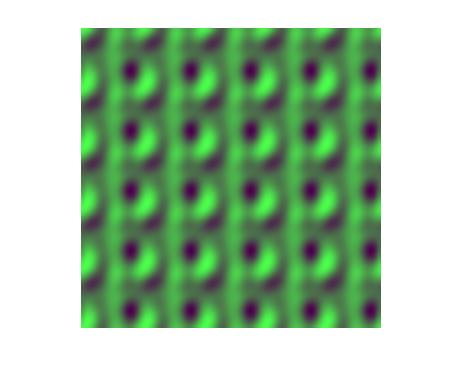
\includegraphics[scale=0.5]{pattern.png}
    \centering
    \caption{An image representation of the structure produced by a system of cells.} 
    \label{pattern}
\end{figure}   
    
The functions in Matlab are written according to the format below:
    \begin{lstlisting}[language=matlab]
        function <output> = name(<arguments>)
            body
        end
    \end{lstlisting}
    
    Note that the output can be a vector, a 2-dimensional array or an abstract structure, meaning that the type of the output value will be given during the execution of the program.  
	\subsection{Modelling morphogenesis}	
    
As explained in Chapter \ref{morphogenesis}, there are several dynamical models of the reaction-diffusion process in morphogenesis. The reaction model has the form $ \dot{x}=F(x) $ and the diffusion model is according to conduction of heat as explained in paragraph \ref{diffusion} with cell interconnections of ring or torus-shaped structures. The Matlab program that was generated to solve such a model has two main parts.
    
The first part is the main function, where the initial conditions are given. Those conditions are the number of cells, the initial concentrations of each chemical compound and the diffusion coefficients. The main function constructs the data structures - which are vectors - and calls the appropriate ODE solver with arguments a function, a column vector (as the initial conditions) and a time span. Other arguments that are used by the ODE algorithm are explained in the next paragraph. Any function can have inside the definition and implementation of another function which is called a nested function.
    
The main purpose of the nested function is to make sure that the implementation of the mathematical model is evaluated correctly. The equations of such a model should be implemented in the nested function in a way that the vector operations are evaluated correctly. From a software development point of view, using a nested function instead of an external one is better, since the defined constants are easily shared from the main to its nested function. An example of a template code for solving ordinary differential equations is shown in Figure \ref{templateCode}.
\begin{figure}[h!]
\begin{center}
    \begin{lstlisting}[language=matlab]
    function out = f()
        %body, initialise constants
        %call an ODE solver, such as ode45, ode23 etc...
        %example:
        [t, x] = ode45(@odefun, [0 100]); 
        %that will solve equations in a time span 0-100 seconds        
        
        plot x in respect to t as x(t(i))=x(i)
            
        function odefun = integration(tspan, init)
            body evaluate equations 
            ode = equation results (column vector)
        end
    end 
    \end{lstlisting}
\caption{Template of Matlab code for solving ODE's.}
\label{templateCode}
\end{center}
\end{figure}
	\subsection{Integrating ordinary differential equations}
    Matlab provides a variety of ODE solver implementations each of them having different properties. Note that there are some constraints in evaluating a model that describes fluid concentrations. The main constraint is that the concentrations must never get a negative value otherwise the model will have no physical meaning.

The ODE-solver used in this project is the \texttt{ode45}. According to the Matlab documentation \texttt{ode45} is for solving non-stiff differential equations of medium order and it is the most common used among the provided ode solvers \cite{MATLAB_2010}.
    
Apart from the ODE arguments shown on line 5 in Figure \ref{templateCode},
    the solver can also be given a structure of options as an extra argument. Options are used to override any default behaviour and explicitly define the constraints that the solver must take into account. The options are declared with the use of the \texttt{odeset} function.
    
The \texttt{odeset} function takes an arbitrary length of arguments. First, a string value is given which represents the key of the parameter that is intended to be overridden following by a real numerical value. For example, any reaction-diffusion model requires that no cell has a negative concentration of any of its morphogens. Thus, the options are constructed with the code below:
    $$ options = odeset('NonNegative',(1:N)); $$
    Where N is the size of the solution vector (cells$\times$morphogens). Note that all matlab ode solvers accept a column vector as the initial conditions and thus extra care should be taken for converting a 2-dimensional array to a column vector and the opposite correctly.
	 
	\subsection{Plotting the results}
    Matlab provides easy to use methods that make plotting graphs convenient. The interest lies on observing graphically the equilibrium points of the system, how the system oscillates and for how long. Thus, plotting the results helps in both the analysis of the system and the testing of the programs.
    \subsubsection{The plot function}
    The ODE solvers can plot a graph by default after the solution is calculated or in real time. However, it is better to store the results of the ODE solvers in arrays to have full control of the data. After executing an ODE solver two matrices can be retrieved; the time vector and an array that can be 1-dimensional or 2-dimensional and contains the results of the variables in each column. This is shown representatively in Table \ref{sampleData}. 

    The plot can be used to show a graph of all the variables according to time or for each variable according to another variable. For example, let $t$ be the time array and $X$ be a 2-dimensional array representing morphogen $X$ values of a cell in each column. Now the row index is associated with the time index according to the relation:
       $$ X[cell][index] = X(t_{index}) $$
    
Executing the plot with arguments $t$ and $X$ as shown in Table \ref{sampleData} will give a plot of a graph containing a number of curves equal to the width of the array $X$. Note that $X$ and $t$ must have an equal number of rows. The generated plot is shown in Figure \ref{samplePlot}.
    
    $$ plot(t, X); $$ 
\begin{table}
\begin{center}
\caption{Data as obtained from integrating a function with input array $X$ of size $4 \times$ \texttt{sizeOf(t)}.}
\label{sampleData}   
\begin{tabular}{| l | l | l | l | l |}
\hline
Time ($t$) & $ X_1 $ & $ X_2 $ & $ X_3 $ & $ X_4 $ \\ \hline
0 & 0.2373 & 0.4588 & 0.9631 & 0.5468 \\ \hline
0.0061 & 0.2402 & 0.4489 & 0.9699 & 0.5194 \\ \hline
0.0122 & 0.2431 & 0.4389 & 0.9767 & 0.4921 \\ \hline
\vdots & \vdots & \vdots & \vdots & \vdots \\ \hline
0.9622 & 0.5530 & -0.7833 & 1.5869 & -2.3828 \\ \hline
0.9811 & 0.5564 & -0.8006 & 1.5916 & -2.4167 \\ \hline
1.0000 & 0.5597 & -0.8177 & 1.5962 & -2.4498 \\ \hline
\end{tabular} 
\end{center}
\end{table}

\begin{figure}[h!]
\centering
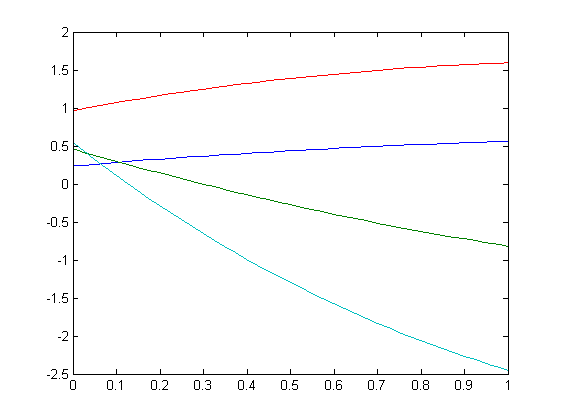
\includegraphics[scale=0.5]{example_plot.png}
\caption{Graph presenting data from Table \ref{sampleData} \label{samplePlot}, Time$\times X$.}
\end{figure}
	\subsection{Creating movies}
    Matlab provides a tool set for creating animated movies. The concept is that a movie is a set of images called frames. Each frame, which is a 3-dimensional image for coloured images, is stored in a 2-dimensional array which contains 3-dimensional frames. Eventually, the result is a 4-dimensional array of size $ F\times X\times Y\times 3 $, with F being the number of frames, $ X\times Y $ the size of each frame and number 3 the vector size of colour values in RGB colour model. 
    
To create a movie, Matlab needs to record images from a figure type window. Thus, for every frame stored, an image must be shown in the same figure window. The function that creates and shows an image out of a 2-3D matrix is called imshow(M), M is the argument that represents a 2-dimensional or 3-dimensional matrix (2D for grey-coloured images, 3D for coloured). Then the function \texttt{getFrame(Figure,window-size)} is called, in order to grab the frame. All frames must be stored in a matrix that was initialised by the function \texttt{moviein(numberOfFrames,Figure,windowSize)}. 
    
Every structure of type `Figure' has an identifier. Thus, keeping the same identifier for the figure that hosts the image from \texttt{imshow()} avoids the creation of many windows. The result is one figure-window that hosts a different image while time passes, resulting in an animated movie show. A structure of type `Figure' is constructed by calling the function \texttt{figure(id)} with \texttt{id} being a natural number. The general function playMovie that was developed can be viewed in Appendix section \ref{playmovie}.

    \subsubsection{Creating the images}
    
Alan Turing states that morphogens are chemical compounds that give certain characteristics to the cells according to their type and concentration \cite{turing_chemical_1990}.
A way to identify and differentiate cells in a computer simulation is to give them different colours according to their morphogen concentrations. Many ideas and combinations were used on how to match morphogen concentrations to different colours. 
    
The first problem in matching morphogen concentrations to colour values is to normalise the concentrations, which are arbitrary real values greater than 0, to real values in the range $ [0,1] $. The Algorithm \ref{colorsmap} describes the colour-mapping procedure.

\begin{algorithm}                      
\caption{Colour mapping}          
\label{colorsmap}                          
\begin{algorithmic}                    
    \STATE{let MORPHOGENS be a 2D array of positive real values}
    \STATE{let MIN be the minimum value in MORPHOGENS}
    \STATE{let MAX be the maximum value in MORPHOGENS}
    \STATE{let an array COLOURS be the same dimensions as the MORPHOGENS array's}    
    \FOR{each VALUE in MORPHOGENS}
        \STATE{NEWVALUE=(VALUE-MIN)/(MAX-MIN)}
        \STATE{add the NEWVALUE to COLOURS}
    \ENDFOR
\end{algorithmic}
\end{algorithm}    

After converting the concentration values in colour values and storing them in a 3-dimensional array, the \texttt{imshow()} method will output a coloured image of a representation of the cells at a certain point in time. This is called a snapshot of the state of the physical system under study.
	\subsection{Producing sound}

    Since models of morphogenesis present an oscillatory behaviour, the wave patterns that are obtained can be mapped into sound waves. A model with continuous/persisting oscillations is the Gizburg-Landau model which involves partial differential equations. The template for computing the mathematical model is given by Aly-Khan Kassam \cite{kassam_solving_2003}.
    
    The morphogen values can be imported directly to the Matlab function \texttt{soundsc(values, sample rate, bit depth)}, that normalises and scales them automatically to sound values. Decreasing the sample rate makes the sound heavier/slower, while higher sample rates make the sound accute. Matlab documentation states that the \texttt{soundsc} function accepts sample rates of the range $[80,10^6]$ \cite{MATLAB_2010} but it is bound on what the sound card on the machine can support.

    The \texttt{soundsc} is available on both Windows and UNIX architectures. The implementation was done on a Linux-based operating system (Fedora 17) and the method used the ALSA drivers to generate sound. 


	\section{Java}
    One of the goals of the project was to identify ideas based on morphogenesis that can be applied to computer science or other engineering problems. Java was chosen as the tool to deliver such solutions, since it can work on many machines and on various operating systems. In addition, Java is more suitable for Object Oriented Programming (OOP) than Matlab. Matlab supports OOP as well, but two main reasons led to the decision of chosing Java over Matlab.
    \begin{enumerate}
    \item The fact that type handling in Java is explicit, helps in a better structural software design, with the use of various patterns as described by the Gang of Four \cite{gamma_design_1998} and GRASP\footnote{GRASP is an acronym for General Responsibility Assignment Software Patterns \cite{larman_applying_2004}} principles \cite{larman_applying_2004} 
resulting to a more understandable, easy to maintain source code.
    \item Matlab is proprietary software and since no explicit Matlab tools are needed, Java is the best way to deliver, develop and expand free, easy-to-implement and use software framework.
    \end{enumerate}

    The solution is broken into two main concepts: Building an ODE solver and a simulation of process management system. The idea is described in paragraph \ref{disch}, Diffusion inspired scheduler.    

	\subsection{Implementing Euler's method}
    
A method for integrating ordinary differential equations is the Euler's method. Euler's method is a first order method \cite{koch_implicit_2000}. Two ways to implement the Euler's method are suggested. The approach that was proposed originally is the explicit method where the time-step is fixed. A more advanced solution is the implementation of implicit methods which change dynamically the time steps to reduce integration errors during steps. 

Euler's method is used for the purpose of the diffusion scheduling. Since there is a limit on the time slice,
the explicit method is used to avoid the disadvantage of increasing the total complexity of the algorithm.
That means that the error per step is proportional to the square of the step size. To approximate the reaction-diffusion model of L-systems, a step of 0.1 time units is considered as suggested and implemented from Christopher G. Jennings, PhD in his work on Turing's Reaction-Diffusion Model of Morphogenesis \cite{website:jennings}. 
    
The method takes the initial values for every variable in a vector $ x_0 $ of size N.
    $$ \dot{x}_0 = \begin{pmatrix}
x_1 \\ 
\vdots \\
x_n \\
\end{pmatrix}
$$ 
    Then, for each time step, starting from $ n = 0 $ it calculates the next state in the next time step.
    $$ \dot{x}_{n+1} = \dot{x}_n + h*f(t_n, \dot{x}_n) $$
    
Where:
\begin{itemize}
\item h is the step size and it should be less than 1.
\item n is the index to the current step.
\end{itemize}    

The algorithm that describes the implementation of the Euler's method is shown in Figure \ref{euleralgo}. The algorithm depends on the function and its number of variables. For that reason, the Template pattern was used to protect the implementation of the Euler's method from function variations. As shown in Appendix \ref{App:AppendixB}, the abstract class AbstractFunction provides a default implementation of an equation. In order to add a new equation, a new class has to be implemented that extends the AbstractFunction. Thus, by the means of inheritance, the variations of different equations are hidden from the ODE solver resulting in a coherent code that does not need to change every time a new equation is added. 

Likewise, ODE solvers can be added, as defined by the ODE interface, without the need of changing the functions since the ODE interface and the AbstractODE is bound to the AbstractFunction. In other words, the principle of GRASP for protecting variations was widely taken into account to construct a well coherent framework.

\begin{algorithm}                      
\caption{Euler's method}          
\label{euleralgo}                          
\begin{algorithmic}
    \STATE{results[0]=initial conditions}                    
    \FOR{i in 1 to number of total steps}
			\STATE{results[i] = results[i-1] + timestep*function()}
    \ENDFOR
    \STATE{return results}
\end{algorithmic}
\end{algorithm}

    \subsection{Process management}

A process is a portion of code that needs to be executed by a processor to accomplish a task. This execution needs time to be completed, proportional to the cycles per second that the processor runs.

The process management is a responsibility of the operating system. Each operating system can have one or more scheduling algorithms to manage the execution of a queue of processes. Modern operating systems, support preemptive multitasking \cite{tanenbaum_modern_2007}. This means, that a process can be paused without its permission and another process can take its place. The scheduling algorithms become more sophisticated in order to handle pseudo-parallelism. The general goal is to keep each process as less idle as possible.

This project explores the behaviour of executing a fixed amount of processes by using a diffusion-inspired scheduler as described in paragraph \ref{disch} 
against other process schedulers. The study is just an introduction to the idea of using the concept of reaction-diffusion to help the algorithm decide on how much time each process must be given each turn.
Each process has the properties described in Figure \ref{processfigure}. 

The processes are arranged in a queue. No new processes are added in the queue and a process is removed from the queue when it exits with a finished or a crash message.
\begin{figure}
\centering
\includegraphics[scale=0.8]{process_figure.png}
\caption{Scheme of a process as handled by the implementation of the process management framework.}
\label{processfigure}
\end{figure}


	\subsection{The scheduling problem}	
\label{schedulers}
The responsibility of a scheduler is to find a way of executing all the processes that seek execution time with maximum efficiency. The term efficient is ambiguous but justifiably so. The goal of a scheduler differs from situation to situation and from system to system. Despite the fact that in a distributed system, prioritising might be less important than executing client requests without the concern of which client should get the response first. There are also some general specifications that a scheduler shall achieve.
Some general goals include:
\begin{itemize}
\item To finish as early as possible.
\item To execute system processes with higher priority.
\item To avoid starvation.
\item To detect deadlocks.
\end{itemize}
Finishing fast is not as crucial as it may seem. It is clear, that the fastest solution in terms of time is to execute the processes serially (assuming all finish at some point). However, the most important concept in a real-world situation is to present pseudo-parallelism, that is to make the processes look that they are being executed in parallel. 
Avoiding starvation is another specification a scheduler has to offer. Assuming that the body of the code under processing does not contain any deadlock situations, then all processes must be executed and finished at some point in time. Thus, each process should take some time in every short amount of cycles. The phenomenon on which a process is not given processing time at all is called starvation. 

Deadlocks are not considered in this project but they should be referenced to avoid conflicts with starvation. A deadlock can occur when two or more processes wait for each other to continue their processing. If this happens, the scheduler will be running those processes forever. Detection of deadlocks is important but is not always the responsibility of the scheduler. Usually, the program that detects deadlocks is called `watchdog' \cite{tanenbaum_modern_2007}. However, it is crucial for a scheduler to work smoothly if deadlocks are detected to avoid wasting time with frozen processes.

The rest of the Chapter describes different scheduler algorithms used to assess the performance of the diffusion-inspired scheduler. These are the random sceduler, the Round-Robin and the priority scheduler. The algorithm of the diffusion-inspired scheduler is also given.
	
\subsubsection{Random scheduler}
The random scheduler picks randomly a process from the queue and executes it for a fixed amount of time units. The pseudo-code is in Algorithm \ref{RandSch} below.


\begin{algorithm}                      
\caption{Random scheduler}          
\label{RandSch}                           % and a label for \ref{} commands later in the document
\begin{algorithmic}                    
    \WHILE {Process queue is not empty}
        \STATE{choose a process at random}
        \STATE{ask the process to run up to a pre-defined number of time units}
        \STATE{get acknowledgment message from process}
        \STATE{get time used by the process}
        \STATE{increase for each other process their idle time}
        \STATE{increase execution time for the process chosen}
        \IF {the process finished}
            \STATE{add execution time, idle time and total time to the scheduler statistics}
            \STATE{remove process from queue}
        
        \ENDIF
    
    \ENDWHILE
    \STATE{display statistics}    
\end{algorithmic}
\end{algorithm}


	\subsubsection{Round Robin scheduler}
The Round Robin scheduler picks serially each process in the queue and executes it for a fixed amount of time units. It guarantees that eventually all processes will be executed and exit. The pseudo-code is shown in the Algorithm \ref{RRSch}.

\begin{algorithm}[H]                      
\caption{Round Robin scheduler}          
\label{RRSch}                           % and a label for \ref{} commands later in the document
\begin{algorithmic}                    
    \WHILE{Process queue is not empty}
        \STATE{choose next process in queue}
        \STATE{ask the process to run up to a pre-defined number of time units}
        \STATE{get acknowledgment message from process}
        \STATE{get time used by the process}
        \STATE{increase for each other process their idle time}
        \STATE{increase execution time for the process chosen}
        \IF{the process finished}
            \STATE{add execution time, idle time and total time to the scheduler statistics}
            \STATE{remove process from queue}
        
        \ENDIF
        \IF{last process in queue}
            \STATE{set pointer back to the start}
        \ENDIF
    
    \ENDWHILE
    \STATE{display statistics}    
\end{algorithmic}
\end{algorithm}
 
	\subsubsection{Priority scheduling}
The priority scheduler is based on the fact that some processes are more important than others. The implementation assigns a random integer 0-39 to each process in the waiting queue. This is the priority of the process; the smaller the number the higher the priority. The scheduler executes serially the processes with the minimum priority number until they are all finished and then moves on to the next minimum priority number until the queue is empty. The pseudo-code is shown in Algorithm \ref{PRSch}.

\begin{algorithm}                      
\caption{Priority scheduler}          
\label{PRSch}                           % and a label for \ref{} commands later in the document
\begin{algorithmic}      
    \STATE{set a priority value from 0-39 for each process}              
    \STATE{set minimum value to 0}    
    \WHILE{Process queue is not empty}
        \IF{a process with priority equal to the minimum value does not exist in the queue} 
        \STATE{find the minimum priority value of a process existing in the process queue}
        \ENDIF        
        \STATE{find the next process with priority value equal to the minimum value}
                
        \STATE{ask the process to run up to a pre-defined number of time units}
        \STATE{get acknowledgment message from process}
        \STATE{get time used by the process}
        \STATE{increase for each other process their idle time}
        \STATE{increase execution time for the process chosen}
        \IF{the process finished}
        \STATE{add execution time, idle time and total time to the scheduler statistics}
        \STATE{remove process from queue}
        
        \ENDIF
    
    \ENDWHILE
    
    \STATE{display statistics}    
\end{algorithmic}
\end{algorithm}
	\subsubsection{Diffusion-inspired scheduler}
\label{disch}
The implementation of the diffusion-inspired scheduler exploits the idea of the Round Robin in an alternative implementation of a weighted Round Robin scheduler. That is, instead of having a fixed amount of time units that a process takes to be executed, the time varies according to Diffusion dynamics. The advantage is that because of diffusion all processes are guaranteed to take some time but not necessarily on every execution round. 

The processes are initially given a certain random time unit value that is in reality the amount of time that it will be given for execution. That amount of time represents the concentration of a morphogen in a physical system of cells, and thus, processes represent cells. The processes are executed for the amount of time units given. After the execution round ends, the reaction-diffusion dynamics are calculated and the system of equations is integrated giving as a result new time units for each process.

An exceptional scenario can be encountered where processes starve. This can happen when all the processes that have a positive time unit are executed and finish, leaving in the queue processes that have 0 time units and are thus unable to diffuse. This is solved by following a simple rule: if a process is called to be executed for 0 time cycles, then it is always executed for one.

A more sophisticated way to avoid starvation is to assign two fixed pseudo-processes to certain places in the queue that have a fixed amount of time units that never change, and thus feeding the rest of the processes avoiding starvation. These scenarios and solutions were not studied. Nevertheless, the fact that starvation did not happen during the experiments points that further investigation is needed. The implemented framework is freely available for expansions and testing various ideas. 

The algorithm of the Diffusion scheduler is provided below (Algorithm \ref{DSch} ).

\begin{algorithm}                      
\caption{Diffusion-inspired scheduler}          
\label{DSch}                           % and a label for \ref{} commands later in the document
\begin{algorithmic}
    \STATE{set randomly time units to a process in a range close to the other ranges

    (alternatively, set equal time units to a process equal to the pre-defined value)}                    
    \WHILE{Process queue is not empty}
        \STATE{choose next process in queue}
        \STATE{ask the process to run up to its given number of time units}
        \STATE{get acknowledgment message from process}
        \STATE{get time used by the process}
        \IF {process used all the time}
        \STATE{set the reaction variable of that process to 0}
        \ENDIF
        \IF {process was last in queue}
        \STATE{set Euler time step to 0.01 as an imaginary time step}
        \STATE{calculate reaction-diffusion differential equations
                by applying Euler's method and assign to each process
                a new amount of time units}

        \ENDIF
        \STATE{increase for each other process their idle time}
        \STATE{increase execution time for the process chosen}
        \IF{the process finished}
        \STATE{add execution time, idle time and total time to the scheduler statistics}
        \STATE{remove process from queue}
        \ENDIF
        \IF{last process in queue}
        \STATE{ set pointer back to the start}
        \ENDIF
    
    \ENDWHILE
    \STATE{display statistics}    
\end{algorithmic}
\end{algorithm}

Development description of the process management framework is given in Chapter \ref{softD}.


\chapter{Applications and results}
\label{results}
The results of this project involve analysis of dynamical systems that describe chemical reactions, cell diffusion and complete  reaction-diffusion process as described in Chapter \ref{morphogenesis}. The latter is a set of linearised and non-linear models. The non-linear models are used to visualise cell structures and to study mutations. Results also show the rationale behind sound generation and some attempts to generate sound. Finally, the statistical information obtained from the scheduling algorithms demonstrate why scheduling using the concept of diffusion is promising. The results are obtained by the software applications that were developed for the project.
	\section{Chemical reactions}
Various chemical reactions were studied to identify how altering various parameters affects their behaviour. The main interest is to observe oscillatory behaviour, if any, and the amount of time needed for a reaction to be completed. Parameters are related to the concentration of each chemical substance, the reaction rate or coefficient which show the amount of each compound needed to produce another compound. 

    The experiments use the chemical reaction equations described by the Michaelis-Menten mechanism as presented in the case study of Stephen Childress \cite{childress_case_2005}. Four chemical substances are involved: one acting as a catalyst (enzyme E) interacting with a chemical substance X for composing the product P. There is a complex chemical compound C as a middle state which breaks into E+X or E+P according to the reaction rates $ k_{-1} $, and $ k_{+2} $ respectively. Note that the index in each rate k indicates the step (backwards, forward) needed to reach a certain state of the reaction.

The chemical reaction equation of the Michaelis-Menten mechanism is:
\begin{equation}
\label{excheq}
 E + X \underset{\underset{k_{-1}} \gets}{\overset{\overset{k_{+1}} \to}{}}  
		 C \overset{k_{+2}} \to E + P
\end{equation}

It is important to note that predictions are made before running an experiment. This helps in both testing and building an understanding of how, in this example, a complex reaction works.

\subsubsection{Prediction}

It is clear from the equation (\ref{excheq}) that the final products will be the enzyme E and the product P. The question arising is how can the maximum possible concentration of P be retrieved at the minimum amount of time? 

The complex compound C breaks into E and X at a rate $ k_{-1} $ into E and P at a rate $ k_{+2} $. When X runs out the reaction stops. Thus, the rate $ k_{+2} $ must be greater or equal to $ k_{-1} $ to accomplish the minimum time.

Table \ref{tableChemExp} shows the parameters of the try-outs for testing the Michaelis-Menten mechanism as described by the chemical equation (\ref{excheq}). 
\begin{table}
\begin{center}
\caption{Parameters used by solving the chemical equation (\ref{excheq}).}
\label{tableChemExp}
    \begin{tabular}{| c | c | c | c | c | c | c | c | c | c | c | c |}
        \hline
         & \multicolumn{4}{| c |}{Initial Concentrations} & \multicolumn{3}{| c |}{Reaction rates} \\ \hline
        Experiment Number & E & X & C & S & $ k_{+1} $ & $ k_{-1} $ & $ k_{+2} $ \\ \hline
        1 & 20 & 20 & 0 & 0 & 0.01 & 0.01 & 0.01 \\ \hline
        2 & 20 & 20 & 0 & 0 & 0.01 & 0.1 & 0.01 \\ \hline
        3 & 20 & 20 & 0 & 0 & 0.01 & 0.01 & 0.1 \\ \hline
        4 & 20 & 20 & 0 & 0 & 0.1 & 0.01 & 0.01 \\ \hline   
    \end{tabular}
\end{center}

\end{table}

\begin{figure}
\centering
\includegraphics[width=15cm, height=10cm]{exp2ch.png}
\caption{Graph showing the behaviour of the chemical reaction when there is a balance in all rates (experiment 1,Table \ref{tableChemExp}).}
\label{exp2ch1}
\end{figure}

\begin{figure}
\centering
\includegraphics[width=15cm, height=10cm]{exp2ch2.png}
\caption{Graph showing how a higher rate of C breaking into X affects Michaelis-Menten mechanism (experiment 2, Table \ref{tableChemExp}).}
\label{exp2ch2}
\end{figure}

\begin{figure}
\centering
\includegraphics[width=15cm, height=10cm]{exp2ch3.png}
\caption{Graph showing how a higher rate of C producing product P affects the Michaelis-Menten mechanism (experiment 3, Table \ref{tableChemExp}).}
\label{exp2ch3}
\end{figure}

\begin{figure}
\centering
\includegraphics[width=15cm, height=10cm]{exp2ch4.png}
\caption{Graph showing how a higher rate of producing C affects the Michaelis-Menten mechanism (experiment 4, Table \ref{tableChemExp}).}
\label{exp2ch4}
\end{figure}

The rationale behind the parameter values is based on discovering how each parameter affects the reaction. Starting with equal reaction rates and then changing only one parameter for each test, the altered behaviour can lead to conclusions which may verify the predictions. If the prediction is proven wrong, then either there is a bug in the code which integrates the differential equations or the logic behind the prediction was false or the mathematical model that described the chemical reaction was wrong.

The results show that, as predicted, that the higher the rate in which C breaks to E and P the less time is needed for chemical X to run out and cause the reaction to end. At the same time the production of E and X must be lower. So, generally the significance at the difference between $ k_{+2} $ and $ k_{-1} $ affects the overall production rate of P. The reaction rate of the production of the complex compound C also affects the time the reaction needs to complete. It can be high enough to satisfy the production rates of both ends. However, if it exceeds a certain threshold it has no effect, as the production rates of X and P are not sufficient to cover the concentration of C. 

The experiments from chemical reactions show that:
\begin{itemize}
\item The chemical reactions can be easily modelled with differential equations.
\item Compounds that break into different chemical substances present more complex behaviours and are closest to produce oscillations rather than equations of the form showed in the first example.
\item Different reaction rates affect the time for the completion of a chemical reaction but values exceeding a threshold may exist that have no effect.
\end{itemize}
   

\section{Diffusion}
Diffusion depends on the interconnections between cells. Two types of interconnection were studied: cells connected in a ring-shaped structure and a torus-shaped connection. The difference between the two is the number of cells each cell is attached to. In a ring, two cells are attached to every other cell. In a torus, four cells are attached to every other cell.

Diffusion was implemented according to the conduction of heat as described in Section \ref{diffusion}.
Experiments were done to identify the role of the parameters of the cells, the diffusion coefficients and the shape of the system. Table \ref{diffexp2} shows the parameters under study and figures \ref{d1}-\ref{d4} show the graph representations of the behaviour of such system.

The expected result after the diffusion process ends is that every cell has the same concentration of a particular morphogen as shown in figures \ref{d1}-\ref{d4}. The diffusion coefficient and the size of the cell affect the fluid flow and therefore smaller cells need more time to diffuse. The properties of a ring structure against a torus structure are also studied.

\begin{table}
\begin{center}
\caption{Parameters used to run tests on diffusion.}
\label{diffexp2}    
\begin{tabular}{| c | c | c | c | c | c |}
        \hline        
        No. & Cell side size & Number of Cells & Shape & Diffusion Coeff. & Initialisation method \\ \hline
        1 & 0.5 & 3 & Ring & 0.1 & Random \\ \hline
        2 & 0.1 & 3 & Ring & 0.1 & Random \\ \hline
        3 & 0.5 & 9 & Ring & 0.1 & Random \\ \hline
        4 & 0.5 & 4 & Torus & 0.1 & Random \\ \hline
    \end{tabular}
\end{center}
\end{table}

\begin{figure}
\centering
\includegraphics[width=15cm, height=10cm]{diffusion1.png}
\caption{Graph showing chemical concentrations during the diffusion process (experiment 1, Table \ref{diffexp2}).}
\label{d1}
\end{figure}


\begin{figure}
\centering
\includegraphics[width=15cm, height=10cm]{diffusion2.png}
\caption{Graph showing how the size of the cells affects the diffusion process (experiment 2, Table \ref{diffexp2}).}
\label{d2}
\end{figure}

\begin{figure}
\centering
\includegraphics[width=15cm, height=10cm]{diffusion3.png}
\caption{Graph showing how the number of the cells affects the diffusion process (experiment 3, Table \ref{diffexp2}).}
\label{d3}
\end{figure}

\begin{figure}
\centering
\includegraphics[width=15cm, height=10cm]{diffusion4.png}
\caption{Graph showing the diffusion process in a torus structure (experiment 4, Table \ref{diffexp2}).}
\label{d4}
\end{figure}

Conclusions obtained from the results of tests 2, 3 and 4 compared to 1 (Table \ref{diffexp2}):
\begin{itemize}
\item Experiment 2 shows that with smaller cells, diffusion needs more time to be completed.
\item Experiment 3 shows that more cells need more time to complete the diffusion process.
\item Experiment 4 shows that a torus structure diffuses faster that a ring one.     
\end{itemize}
		
\section{Reaction-diffusion}
    Reaction-diffusion models can be considered as complete models of morphogenesis. They result from merging reaction and diffusion models. Depending on the type of the function, linear or non-linear, that describes a chemical reaction, the models are categorised into linear or non-linear.
    
The linearised model that is tested in Section \ref{resLinear} produces negative solutions as well. Negative solutions are not accepted when working with chemical substances, since a negative concentration does not have a physical meaning. There is an option for forcing the ODE solver to always produce non-negative solutions. However, this results in unstable behaviour. Nevertheless, as explained in Section \ref{linsys} the goal is to approximate the behaviour of a system near the equilibrium points. In other words, the study is about the qualitative behaviour of the system rather than the quantitative one.

Modelling with non-linear systems gives an approximation closer to reality since chemical substances can't be negative. Results for non-linear systems include image snapshots of the cell structure at particular time points.

    
\subsection{Implementing and testing with linearised models}
\label{resLinear}
The linear system that was studied is proposed by Alan Turing \cite{turing_chemical_1990} and analysed in the case study of Stephen Childress \cite{childress_case_2005}. The main interest lies on the stability conditions. The equation is of the form:
$$ \dot{x} = Ax $$
Where A is the Jacobian matrix evaluated at the equilibrium point as described in  \ref{linsys} and has size $ N\times N $.
The case studies a system with 2 morphogens. 
$$ N=2,$$
$$ A \in \mathbb{R}^{2\times 2} $$

The stability conditions are computed by finding the roots of the characteristic equation obtained from equation (\ref{char}) and analysed in \cite[p.~5]{childress_case_2005} computing the conditions shown in equation (\ref{conditionsA}).
\begin{equation}
\label{jacobian}
A= 
\begin{pmatrix}
        a_{11} & a_{12} \\
        a_{21} & a_{22} \\
\end{pmatrix}
\end{equation}

\begin{equation}
\label{char}
det(A-\lambda I) = 0 
\end{equation}

$$a_{11} + a_{22} < 0,$$
\begin{equation}
\label{conditionsA}  
 a_{11}a_{22} - a_{12}a_{21} > 0
\end{equation}


In other words, the linearised matrix can have several random forms, but always satisfy the given conditions in \ref{conditionsA}. The program in Appendix Section \ref{initialisea} is responsible for the generation of such random matrices. Table \ref{linexp} shows the different values of the matrix. The Figures \ref{l1}-\ref{l4} show the behaviour of the system. Note that the Jacobian matrix is used to approximate the behavior of the reaction process. Merging the corresponding matrix with the diffusion in a ring of cells from equation (\ref{diffeq}), the system becomes as shown by equation (\ref{lrdm}).

\begin{equation}
\label{lrdm}
\dot{x}_i = Ax_i + \begin{pmatrix}
\delta^2d_1 & 0 \\
0 & \delta^2d_2 \\
\end{pmatrix}(x_{leftof(i)} - 2x_i + x_{rightof(i)})
\end{equation}

\begin{table}
\begin{center}
\caption{Experiments using the Jacobian matrix and diffusion for modelling the process of reaction-diffusion in a ring of cells.}
\label{linexp}
\begin{tabular}{| c | c | c | c | c | c |}
\hline
No. & A & No. of cells & Diffusion included & Initial state & Satisfies conditions\\ \hline
1 & $ \begin{pmatrix}
        0.6171 & 0.8244 \\
        -1.6432 & -0.8824 \\
\end{pmatrix} $ & 3 & Yes & Random & Yes\\ \hline
2 & $\begin{pmatrix}
        0.6834 & 0.4423 \\
        -2.1634 & -1.3875 \\
\end{pmatrix} $ & 3 & Yes & Random & Yes\\ \hline
3 & $\begin{pmatrix}
        -1.6364 & 0.8824 \\
        -0.5 & -0.312 \\
\end{pmatrix} $ & 3 & Yes & Random & No \\ \hline
4 & $ \begin{pmatrix}
        0.6171 & 0.8244 \\
       -1.6432 & -0.8824 \\
\end{pmatrix} $ & 3 & No & Random & Yes \\ \hline
\end{tabular}
\end{center}
\end{table}

\begin{figure}
\centering
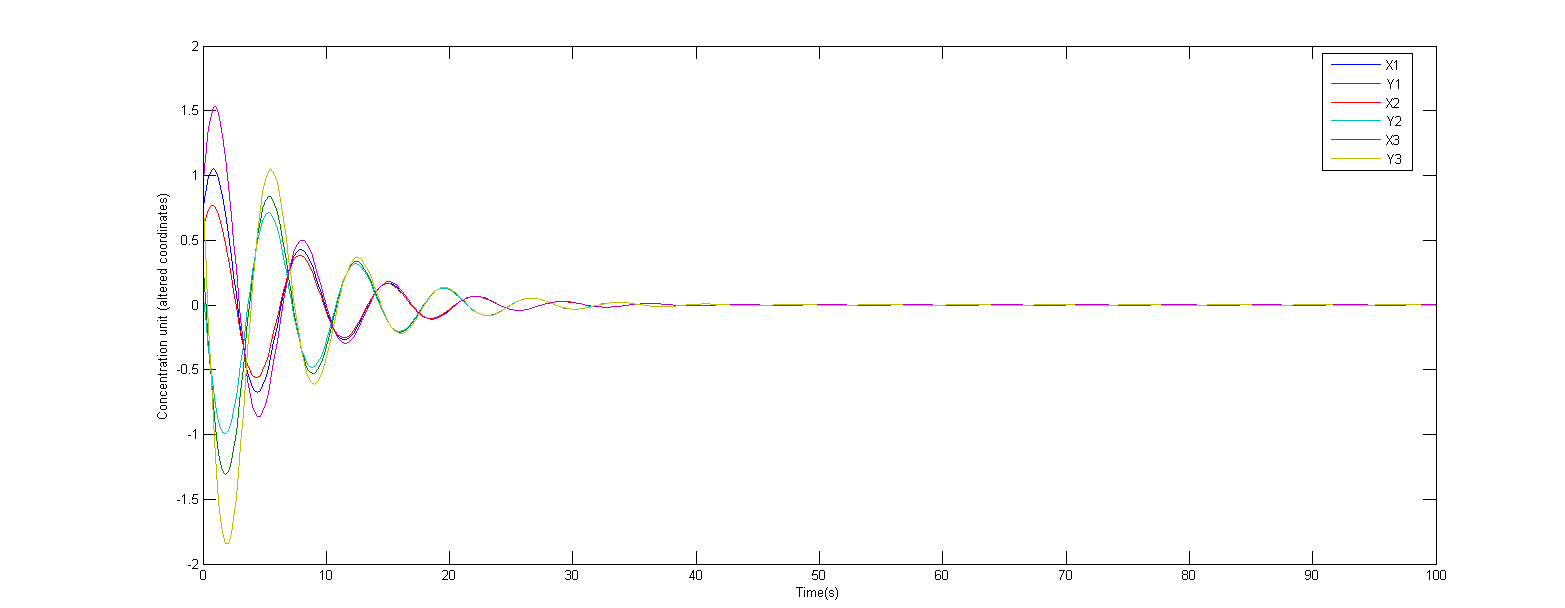
\includegraphics[width=15cm, height=10cm]{l1.png}
\caption{Graph showing the behaviour of a linear reaction-diffusion system (experiment 1, Table \ref{linexp}).}
\label{l1}
\end{figure}

\begin{figure}
\centering
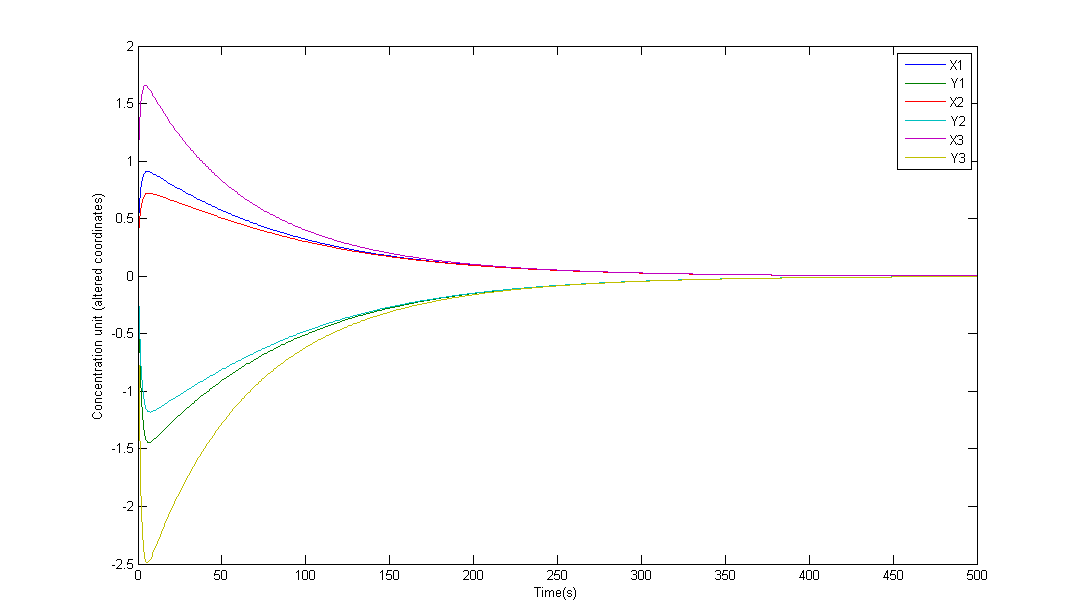
\includegraphics[width=15cm, height=10cm]{l2.png}
\caption{Graph showing the behaviour of a linear reaction-diffusion system with different values of the Jacobian matrix (experiment 2, Table \ref{linexp}).}
\label{l2}
\end{figure}

\begin{figure}
\centering
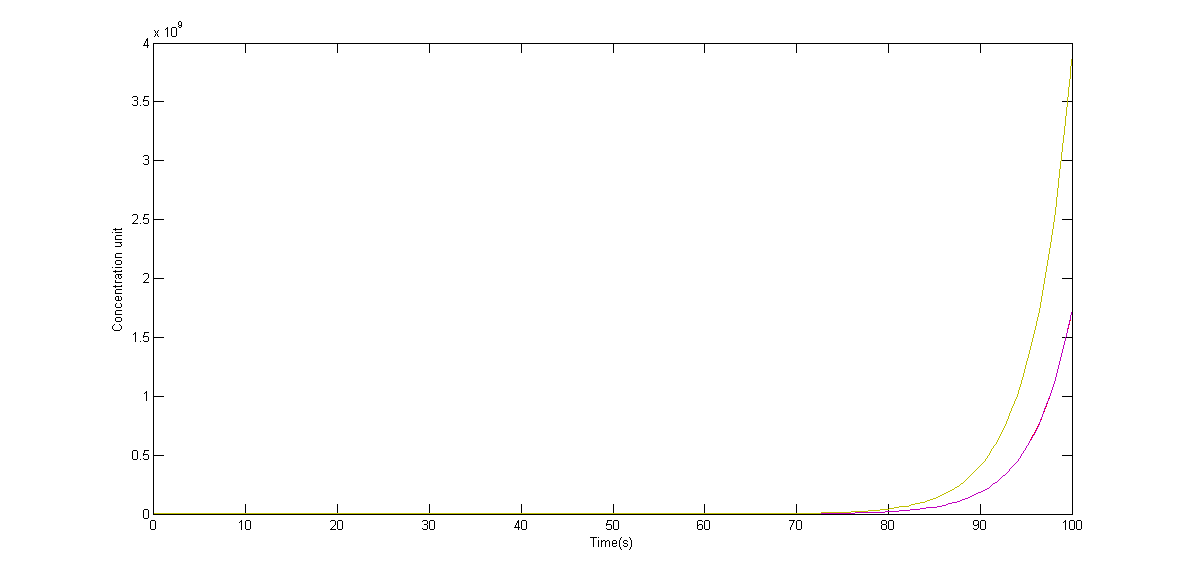
\includegraphics[width=15cm, height=10cm]{l3.png}
\caption{Graph showing that a linearised reaction-diffusion system is unstable if stability conditions are not satisfied (experiment 3 from Table \ref{linexp}).}
\label{l3}
\end{figure}

\begin{figure}
\centering
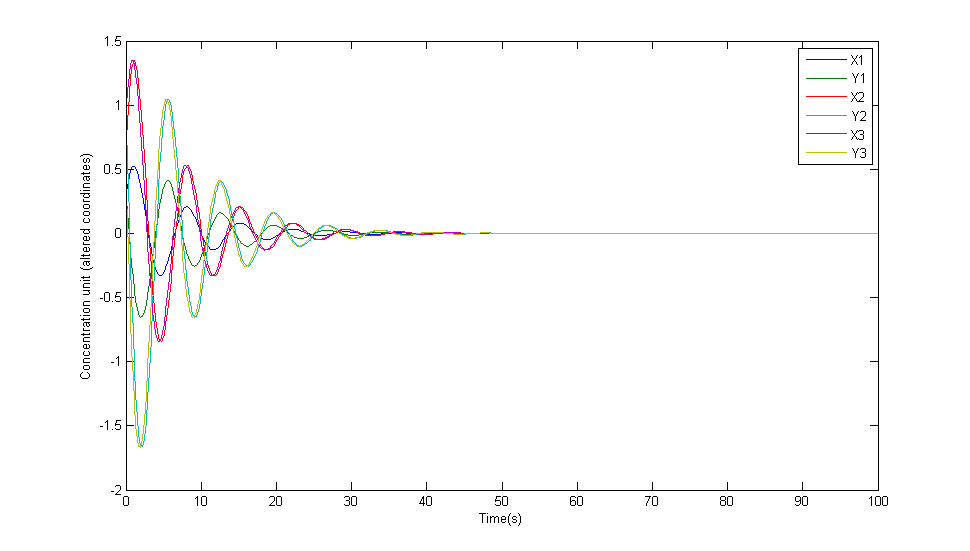
\includegraphics[width=15cm, height=10cm]{l4.png}
\caption{Graph showing the same linear system as in experiment 1 but without diffusion (experiment 4, Table \ref{linexp}).}
\label{l4}
\end{figure}

The experiments show that:
\begin{itemize}
\item The absence of diffusion as opposed in experiment 4 of table \ref{linexp} does not affect the oscillatory behaviour.
\item Not satisfying the stability conditions leads to an unstable system with infinity values, as shown in test 3 of table \ref{linexp}.
\end{itemize}

Results do not prove or show regarding the way that diffusion affects the system. Trying to perform the same tests by changing the diffusion coefficients only is shown in Table \ref{diffLexp} and figures \ref{ld1}, \ref{ld2} opposed to \ref{l1} and \ref{l2} respectively. 

\begin{table}
\caption{Experiments on how a linear system is affected from diffusion.}
\label{diffLexp} 
\begin{center}
\begin{tabular}{| c | c | c | c | c |}
\hline
No. & A & No. of cells & {Diffusion coefficients (M)} & Initial state\\ \hline
1 & $ \begin{pmatrix}
        0.6171 & 0.8244 \\
        -1.6432 & -0.8824 \\
\end{pmatrix} $ & 3 & 
$ \begin{pmatrix}
        0.025 & 0 \\
        0 & 0.05 \\
\end{pmatrix} $
 & Random \\ \hline


2 & $ \begin{pmatrix}
        0.6171 & 0.8244 \\
        -1.6432 & -0.8824 \\
\end{pmatrix} $ & 3 & 
$ \begin{pmatrix}
        2.5 & 0 \\
        0 & 5 \\
\end{pmatrix} $
 & Random \\ \hline


3 & $\begin{pmatrix}
        0.6834 & 0.4423 \\
        -2.1634 & -1.3875 \\
\end{pmatrix} $ & 3 & 
$ \begin{pmatrix}
        0.025 & 0 \\
        0 & 0.05 \\
\end{pmatrix} $ 
& Random \\ \hline


4 & $\begin{pmatrix}
        0.6834 & 0.4423 \\
        -2.1634 & -1.3875 \\
\end{pmatrix} $ & 3 & 
$ \begin{pmatrix}
        40 & 0 \\
        0 & 80 \\
\end{pmatrix} $ 
& Random \\ \hline
\end{tabular}
\end{center}
\end{table}


\begin{figure}
\centering
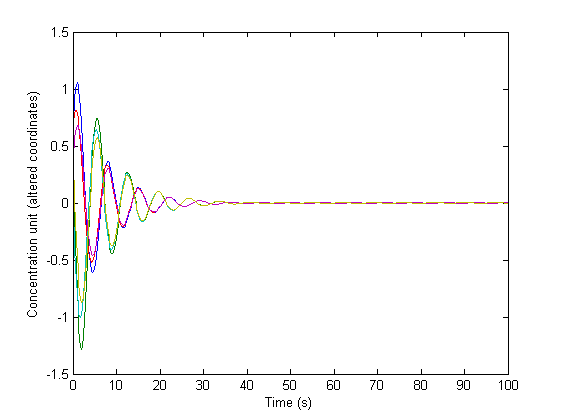
\includegraphics[width=15cm, height=10cm]{ld1.png}
\caption{Graph showing how the behaviour of the linear system differantiates with large diffusion coefficients (experiment 2, Table \ref{diffLexp} opposed to experiment 1, Figure \ref{l1}).}
\label{ld1}
\end{figure}

\begin{figure}
\centering
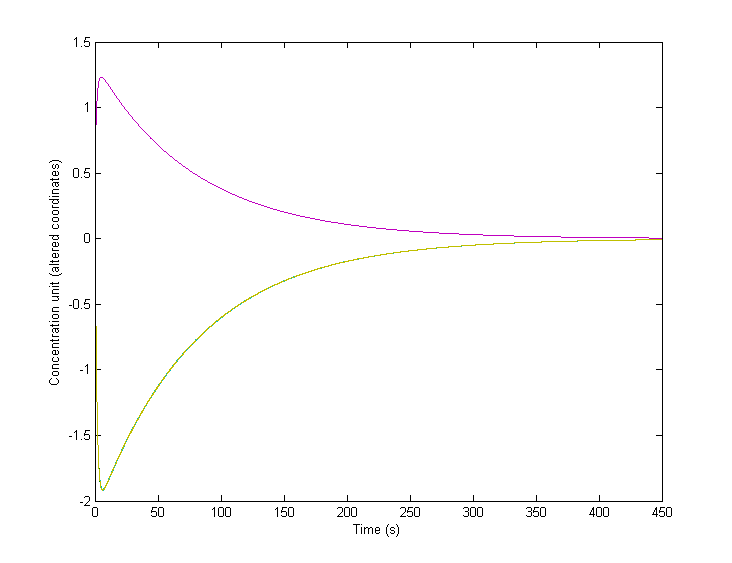
\includegraphics[width=15cm, height=10cm]{ld2.png}
\caption{Graph showing how the behaviour of the linear system differantiates with very large diffusion coefficients (experiment 4, Table \ref{diffLexp} opposed to experiment 3, figure \ref{l2}).}
\label{ld2}
\end{figure}

Notice now that only two colours are visible in the graph \ref{l2}. That means that morphogen concentrations in cells are equal and thus, with high diffusion coefficients (40 and 80) all cells rapidly become identical. This means that large diffusion coefficients must be avoided in order to differentiate cells.

The general conclusion is that diffusion is very important in morphogenesis and has a high impact on the behaviour of the system. Despite the fact that graphs show identical behaviour, it should not be neglected that the purpose of the project is to generate software applications that present how cells create structures. Cells must have properties that differentiate one-another. By setting a large diffusion coefficient value, cells may become quickly identical and the internal chemical reactions will not lead into different results. The choice of diffusion coefficients is therefore critical.


\subsection{Non-linear models}
\label{resnonlinear}
The non-linear models discussed in Chapter \ref{morphogenesis} were used to the final software solutions. The main purpose was to show how cells are organising and form structures out of a random chaotic state. The results are shown in images that represent the structure of the system. Those images are snapshots of the system at time zero, middle and final point snapshots are arranged in a timeline. 

Table \ref{rdtable} shows the parameters and the models that were used. Notice that diffusion coefficients and the number of cells affect the structure of the system. 

\begin{table}
\begin{center}
\caption{Experiments of non-linear models with various parameters.}
\label{rdtable}
\begin{tabular}{| c | c | c | c | c |}
\hline
No. & Model & Parameters & Diffusion Coefficients & Number of Cells \\ \hline
1 & L-Systems & None & $ D_u=1.6, D_v=6 $ & 6400 \\ \hline
2 & L-Systems & None & $ D_u=1.6 $,$ D_v=6 $ & 22500 \\ \hline
3 & L-Systems & None & $ D_u=3.5 $, $ D_v=16 $ & 6400 \\ \hline
4 & L-Systems & None & $ D_u=2 $, $ D_v=5 $ & 6400 \\ \hline
5 & Gray Scott & $ F=40 $,$ k=60 $ & $ D_u=1 $, $ D_v=16 $ & 22500 \\ \hline
6 & Gray Scott & $ F=30 $,$ k=40 $ & $ D_u=1 $, $ D_v=16 $ & 22500 \\ \hline
\end{tabular}
\end{center}
\end{table}

\begin{figure}
\begin{center}
\includegraphics[width=4cm, height=4cm]{rd11.png}
\includegraphics[width=4cm, height=4cm]{rd12.png}
\includegraphics[width=4cm, height=4cm]{rd13.png}
\end{center}
\caption{Initial, middle and final snapshots of the structure of the L-systems of experiment No. 1, Table \ref{rdtable}.}
\label{rd1}
\end{figure}

\begin{figure}
\begin{center}
\includegraphics[width=4cm, height=4cm]{rd21.png}
\includegraphics[width=4cm, height=4cm]{rd22.png}
\includegraphics[width=4cm, height=4cm]{rd23.png}
\end{center}
\caption{Initial, middle and final snapshots of the structure of the L-systems with more cells as shown in experiment 2, Table \ref{rdtable}.}
\label{rd2}
\end{figure}

\begin{figure}
\begin{center}
\includegraphics[width=4cm, height=4cm]{rd31.png}
\includegraphics[width=4cm, height=4cm]{rd32.png}
\includegraphics[width=4cm, height=4cm]{rd33.png}
\end{center}
\caption{Initial, middle and final snapshots of the structure of the L-systems with different diffusion coefficients (experiment 3, Table \ref{rdtable}).}
\label{rd3}
\end{figure}

\begin{figure}
\begin{center}
\includegraphics[width=4cm, height=4cm]{rd41.png}
\includegraphics[width=4cm, height=4cm]{rd42.png}
\includegraphics[width=4cm, height=4cm]{rd43.png}
\end{center}
\caption{Initial, middle and final snapshots of the structure of the L-systems with different diffusion coefficients (experiment 4, Table \ref{rdtable}).}
\label{rd4}
\end{figure}

\begin{figure}
\begin{center}
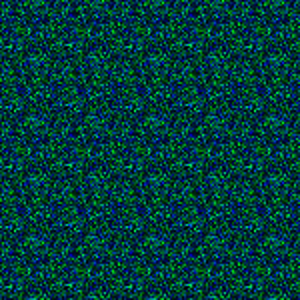
\includegraphics[width=4cm, height=4cm]{gs11.png}
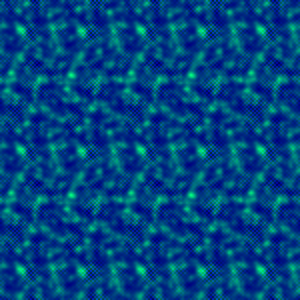
\includegraphics[width=4cm, height=4cm]{gs12.png}
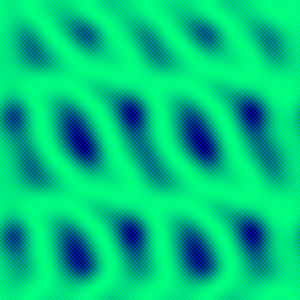
\includegraphics[width=4cm, height=4cm]{gs13.png}
\end{center}
\caption{Initial, middle and final snapshots of the structure of the Gray-Scott model with parameters shown in experiment No.5, Table \ref{rdtable}.}
\label{gs1}
\end{figure}

\begin{figure}
\begin{center}
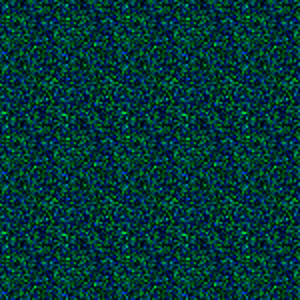
\includegraphics[width=4cm, height=4cm]{gs21.png}
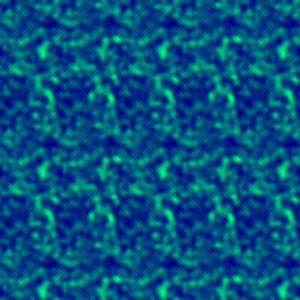
\includegraphics[width=4cm, height=4cm]{gs22.png}
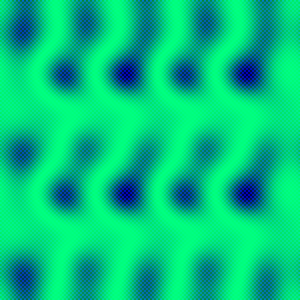
\includegraphics[width=4cm, height=4cm]{gs23.png}
\end{center}
\caption{Initial, middle and final snapshots of the structure of the Gray-Scott model with different reaction rates (experiment No.5, Table \ref{rdtable}).}
\label{gs2}
\end{figure}

As shown in Figures \ref{rd1}-\ref{gs2}, a variety of different structures is obtained. The cells start with a randomly initialised state, but they form shapes and patterns progressively in time.



\subsection{Introducing mutation}

A physical system in the real world is never isolated. External factors or random events might affect the cells by changing their state. This phenomenon is called mutation and one of the reasons, for example, for producing cancerous masses in advanced biological organisms or causing changes of characteristics (for instance, change in the eye colour). In some organisms, controlled mutations may have desirable effects. In agriculture, grafting takes place in plants to make them produce better fruit \cite{nelson_principles_2007}. Mutation occurs under different circumstances, but the concept remains the same; the behaviour of a system is changed by altering some of its properties.

A study on altering the system randomly after its development is proposed. The process is that the system is left to evolve for a specific amount of time. Then, random perturbations change some cells by altering their morphogen concentrations and the system is integrated again. The purpose is to find at what mutation probabilities the structure of the system is changed dramatically beyond recovery.

This can be done by observing the structures prior to and following mutation. Due to the colour mapping, a single cell mutation may lead to the false conclusion that the structure changed rapidly but this is not the case. What one should observe is whether the change in some cells can be absorbed by the system and if the system recovers to its previous structure.

\begin{table}
\begin{center}
\caption{Showing the effect of mutation on different probabilities.}
\label{muttable}
\begin{tabular}{| c | c | c | c | c |}
\hline
No. & Diffusion Coefficients & Number of Cells & Mutation Probability & Number of mutated cells \\ \hline
1 & $ D_u=1.6, D_v=6 $ & 3600 & 0.001 & 2 \\ \hline
2 & $ D_u=1.6, D_v=6 $ & 3600 & 0.01 & 39 \\ \hline
\end{tabular}
\end{center}
\end{table}

\begin{figure}
\begin{center}
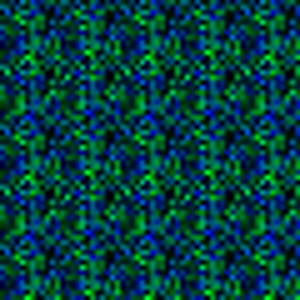
\includegraphics[width=4cm, height=4cm]{st1.png}
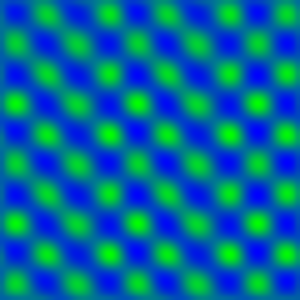
\includegraphics[width=4cm, height=4cm]{bm1.png}
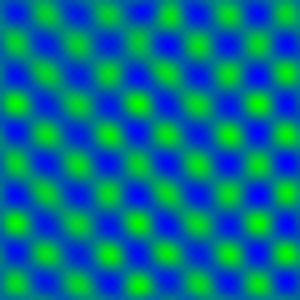
\includegraphics[width=4cm, height=4cm]{am1.png}
\end{center}
\caption{Initial state, final structure before mutation , and recovered structure after mutation with mutation probability 0.001 (experiment 1, Table \ref{muttable}).}
\label{mut1}
\end{figure}

\begin{figure}
\begin{center}
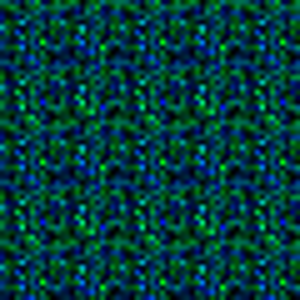
\includegraphics[width=4cm, height=4cm]{st2.png}
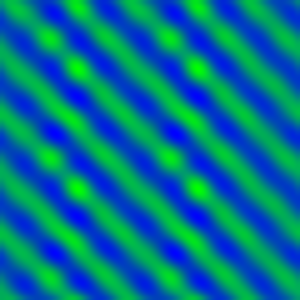
\includegraphics[width=4cm, height=4cm]{bm2.png}
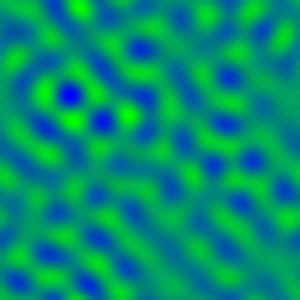
\includegraphics[width=4cm, height=4cm]{am2.png}
\end{center}
\caption{Initial state, final structure before and after mutation showing that with probability 0.01 the structure changes (experiment 2, Table \ref{muttable}).}
\label{mut2}
\end{figure}

The results show that a probability of cell mutation equal to 0.01 is sufficient to alter the final structure of a system. 

More ideas arise on how to experiment with mutation. One is to find the highest probability at which a system can recover. As shown, a probability of 0.01 caused the structure of the system to change while the probability of 0.001 did not affect the system. What may be the threshold that brings the system to its limit?

Another idea would be to simulate the method of grafting. In this method, a tissue is taken from a plant and is inserted into another one. That process may transform, for example, a part of a mandarin tree to become an orange tree. A similar approach can be used to visualise this concept. A way of accomplishing this could be to generate two structures. In practice, the structures are matrices, in theory they are systems of cells. Then, take from the two structures a portion (a column, a row, or a small square portion) of each and substitute them. How will each structure be after integration? This is an interesting experiment that expands the results of this section.


	\section{Producing sound}
\label{glsound}
Mathematical models of morphogenesis have oscillatory behaviour. Thus, they share a common behaviour with sound. The sinusoidal waves of a mathematical reaction-diffusion model can be converted into frequency spectra and then sound may be produced by driving the spectra values to the sound card.

A mathematical model that presents continuous waves is needed. The Gizburg-Landau was used as was analysed and implemented by Aly-Khan Kassam \cite{kassam_solving_2003}
Figure \ref{gl}
shows the pattern that this model generates.    

There are various ways for extracting frequency spectra values from the waves that the Gizburg-Landau model generates. The problem is the same with colour values: to find the right way for mapping the morphogen concentrations into frequency values. The method that was followed was to get the mean of the morphogen concentrations for each point in time. The result is shown in Figure \ref{soundspectra}.


\begin{figure}
\centering
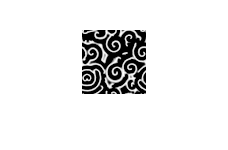
\includegraphics{gl.png}
\caption{Pattern produced by the Gizburg-Landau model.}
\label{gl}
\end{figure}

\begin{figure}
\centering
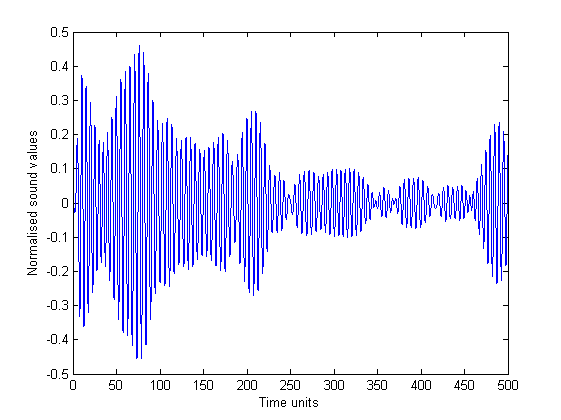
\includegraphics[scale=0.7]{sound_spectra.png}
\caption{Sound spectra by calculating the mean values of the morphogens.}
\label{soundspectra}
\end{figure}


	\section{Comparing schedulers}
\label{sca}
The scheduling solution described in Section \ref{schedulers}
involved four schedulers. The random scheduler, a priority scheduler, the Round Robin Scheduler and the project-related diffusion-scheduler. The results show a similar performance of the Round Robin and the Diffusion scheduler. As shown in the bar graph Figures \ref{schh}, \ref{schk}, \ref{fiveschk}, \ref{fifteenschk}
the diffusion-inspired scheduler can execute processes faster than the other schedulers.

However, the main problem is the complexity of the implementation of the Euler's method inside the scheduler which demotivates the import of the diffusion scheduler to a real operating system. Further study can be made on how it can be imported to a distributed system by handling concurrency.

Table \ref{schtable} shows a short amount of testing and statistical analysis which proves why further study on diffusion-inspired scheduling is needed.  

\begin{table}
\caption{Experiment parameters for testing the diffusion-inspired scheduler against other schedulers.}
\label{schtable}
\begin{center}
\begin{tabular}{| c | c | c |}
\hline
No. & Diffusion Coefficient &  Number of Processes \\ \hline
1 & 1 & 100 \\ \hline
2 & 1 & 1000 \\ \hline
3 & 5 & 1000 \\ \hline
4 & 15 & 1000 \\ \hline
\end{tabular}
\end{center}
\end{table}

\begin{figure}
\centering
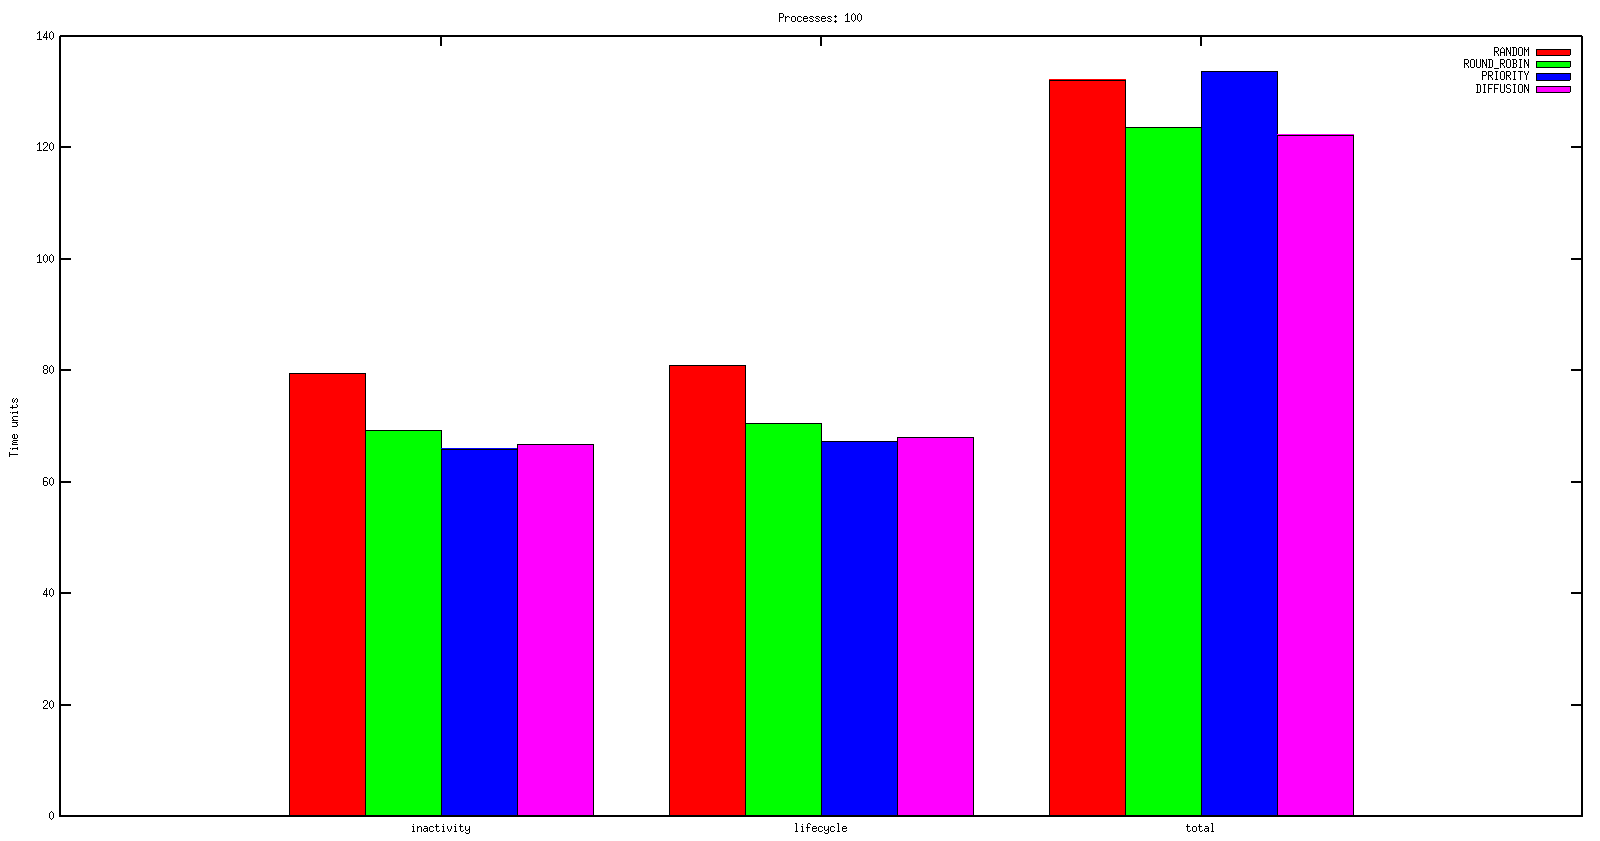
\includegraphics[scale=0.3]{sch100.png}
\caption{Comparison of the scheduler implementations with 100 processes in the queue (experiment No. 1 of Table \ref{schtable}).}
\label{schh}
\end{figure}

\begin{figure}
\centering
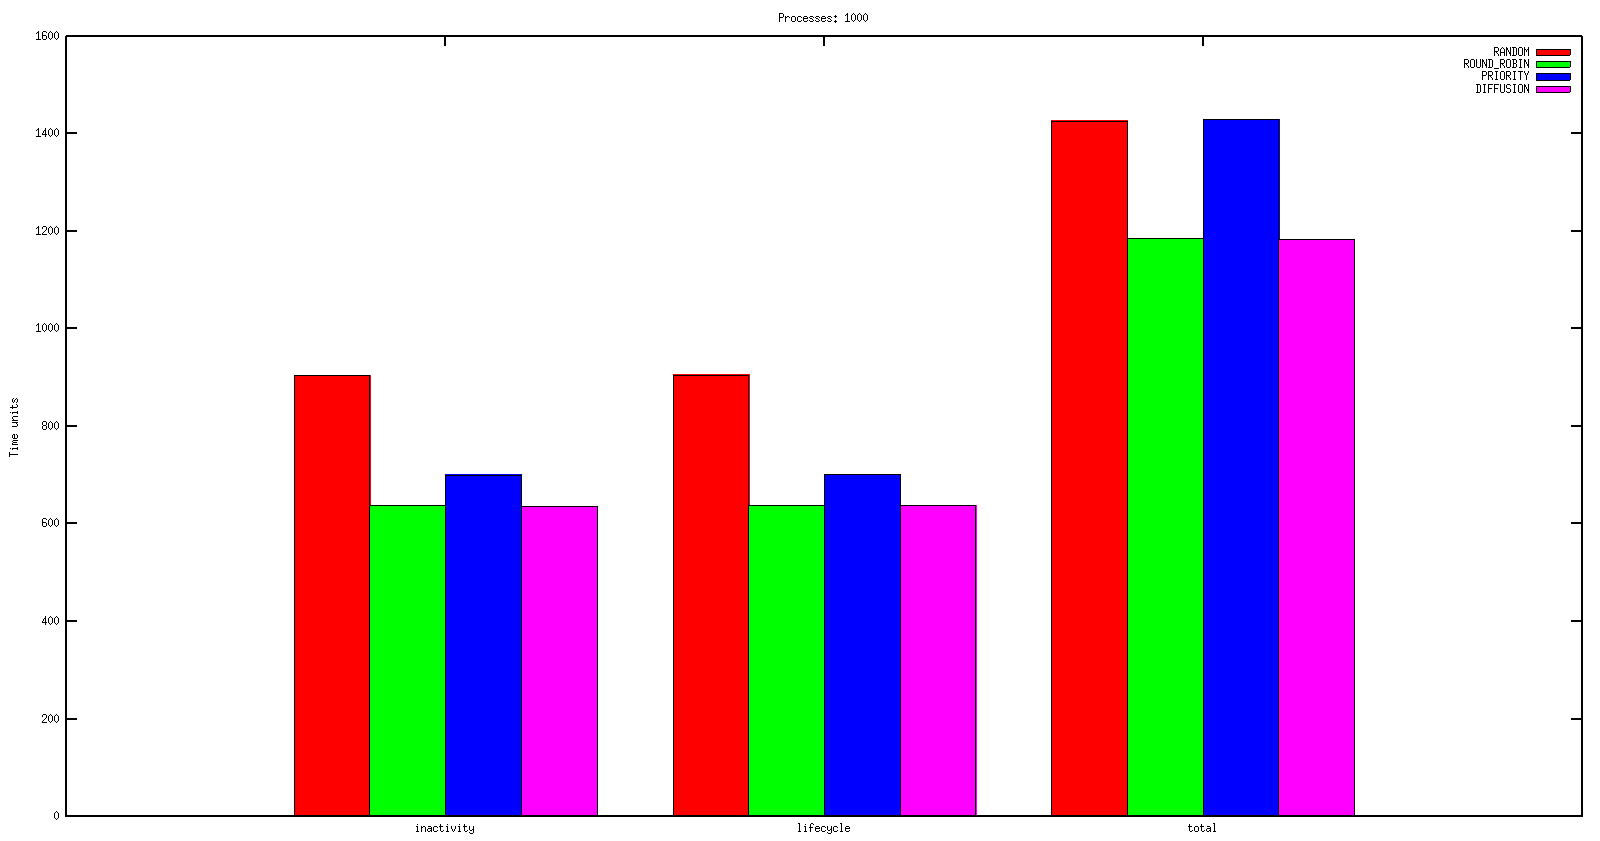
\includegraphics[scale=0.3]{sch1000.png}
\caption{Comparison of the scheduler implementations with 1000 processes in the queue (experiment No. 2 of Table \ref{schtable}).}
\label{schk}
\end{figure}

\begin{figure}
\centering
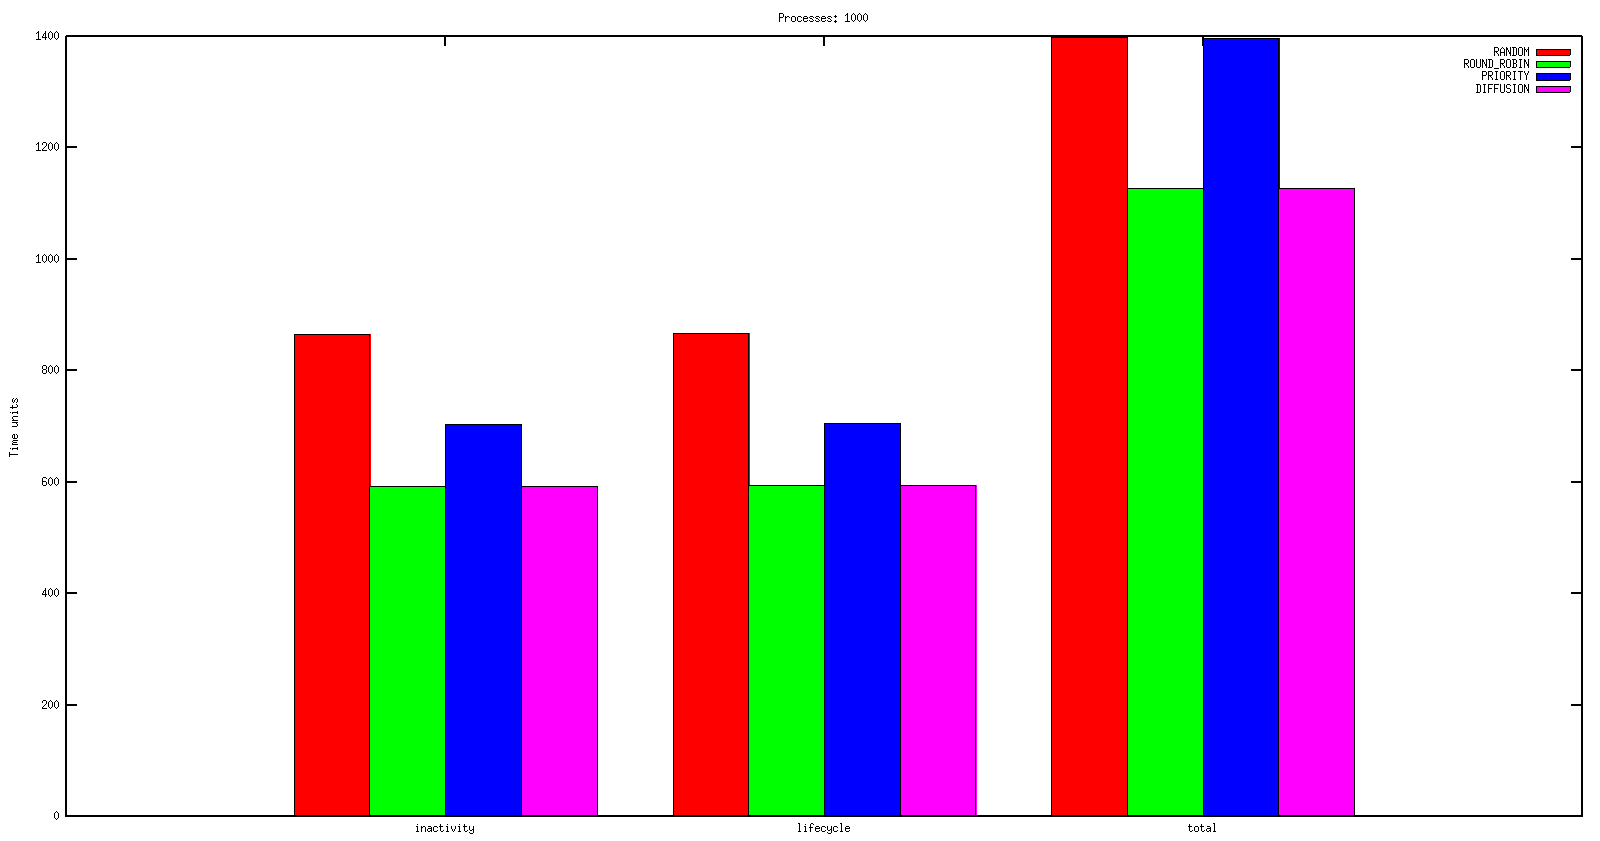
\includegraphics[scale=0.3]{5sch1000.png}
\caption{Comparison of the scheduler implementations with 1000 processes in the queue and a different diffusion coefficient (5) for the diffusion-inspired scheduler (experiment No. 3 of Table \ref{schtable}).}
\label{fiveschk}
\end{figure}

\begin{figure}
\centering
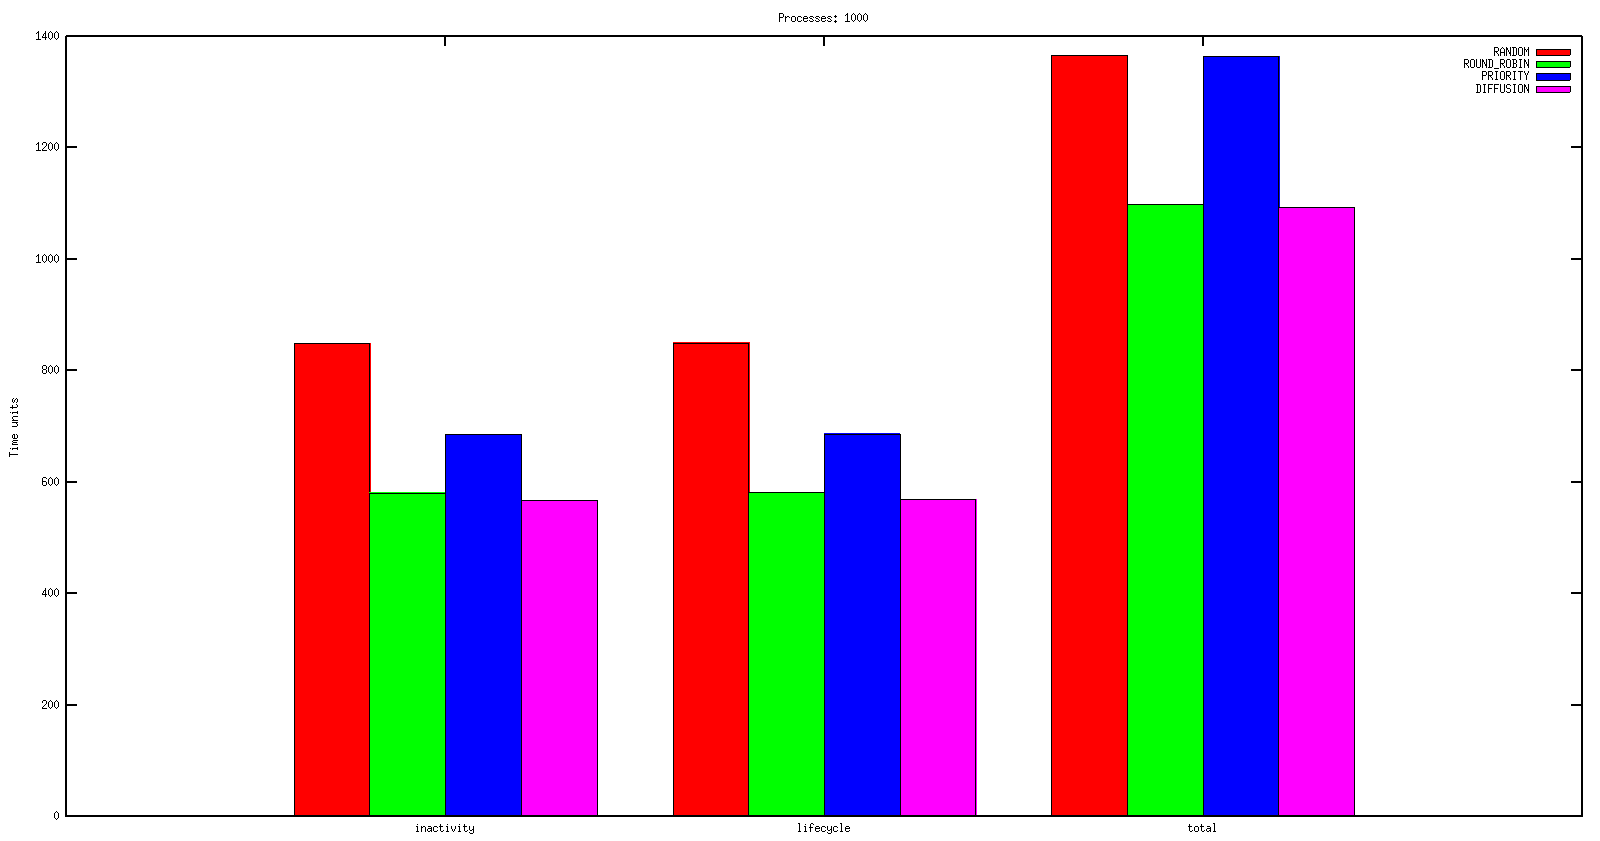
\includegraphics[scale=0.3]{15sch1000.png}
\caption{Comparison of the scheduler implementations with 1000 processes in the queue and the diffusion coefficient of the diffusion-inspired scheduler being 15 (experiment No. 4 of Table \ref{schtable}).}
\label{fifteenschk}
\end{figure}
		


\chapter{Software development}
\label{softD}
The software development process involved implementing simulations for the mathematical models described in Chapter \ref{morphogenesis}, 
testing that involved a basic mathematical analysis of each model and documentation of the work.
The methodologies that were followed during the project can be used as a reference for the reader in order to follow or improve such a method for future research or a related project. It can also be used as a method of understanding the coding structure and then expanding the ideas that are introduced in this project.

\section{Model simulations}
The main deliverable concerning model simulations is a Matlab application. The methodology is discussed to help the reader in using the application and its source code. It might also be used as a guide for solving similar problems.  

\subsection{Code structure}
The code has three main components:
\begin{itemize}
\item The main function that prompts the user to initialise certain parameters of the model, such as the number of cells and the amount of time to be used in integrating the equations.
\item A nested function in the body of the main function that calculates the equations of a certain model. Whether it can be uncoupled from the main function is debatable; it is easier to share variables from the main function to the nested one.
\item Global external functions that can be used by any application and can be easily imported by anyone who is interested in using them. Examples of such functions are the \texttt{playMovie} and \texttt{scaleColors}.
\end{itemize}
Globally available functions are shown in appendix\ref{App:AppendixA}.


\subsection{Testing}

Testing mathematical models is challenging. In general, software testing is done by comparing the output of a body of code with hard-coded data (that is, the expected output). For testing a mathematical model, an analysis of that model needs to be done first, in order to identify what behaviour is expected. The analysis can be automated with the use of the symbolic computational capabilities of Matlab \cite{MATLAB_2010} or Mathematica \cite{mathematica}.

Testing of function implementation that do not involve integration of a system of equations is done in a traditional approach; the output results of a function for certain inputs are compared to expected outputs for those input values. 
The \texttt{scaleColors} function is a crucial function to the system, since it is a key part in mapping the morphogen concentrations to color interpreted values. It takes an array of morphogen concentrations and normalises their values to the range of $[0,1]$ according to the maximum and minimum concentrations. 
%An example of the testing procedure on this function is provided on the table x below. %TODO

%TODO put table here
\subsection{Documentation}

Documentation of the work is presented in HTML format. The purpose of documenting the Matlab functions is to provide a quick reference of the functions implemented, their arguments and their interdependence. 
In order to automate the process of documentation a Bash script was created that gets a set of Matlab files and creates HTML files that provide information of the functions in each file (see bash scripts \ref{matdocpages} and \ref{matdoc}). 

\section{Process scheduling}

The deliverable is a framework written in Java that can be used for:
\begin{enumerate}
\item Creating Scheduler algorithms.
\item Implementing ODE solvers.
\item Defining mathematical models.
\item Running and retrieving statistical results for each scheduler.
\end{enumerate}
An additional tool written in bash script and gnuplot script is provided for converting the statistical information generated by the Java implementation into bar graphs. All scripts can be found in Appendix \ref{App:AppendixC}. %TODO other helpful scripts
%TODO put Appendix 

\subsection{Methodology}
The framework is meant to be used by anyone that wants to experiment with the idea of scheduling by solving differential equations. Thus, the use of software design patterns was essential in order to make the code readable and easy to be expanded. Documentation was generated with proper commenting of the code and then the use of \texttt{javadoc} \cite{javadoc} and testing was done with graph generation by using gnuplot scripts.

\subsection{Code structure}
All class files are included in a single package. The naming of the files is based on software design patterns. Testing was done by the use of bash scripts and the use of the test class "TestScheduler" for the schedulers. The graphs for analysing the effectiveness of each algorithms were generated with the program gnuplot and bash scripts to create data files for the gnuplot scripts.  

\subsubsection{Software design patterns}
A fair amount of software design patterns were used in order to make the code more readable and easier to maintain. %TODO
The patterns were used in reference of the `Gang of Four' \cite{gamma_design_1998} and GRASP \cite{larman_applying_2004}.

The Template pattern was used to protect variations among various ODE solvers, equations/functions and schedulers. A default implementation is given by either an interface or an abstract class and every class-object that provides a specific implementation extends that interface or abstract class. This helps in extending the framework with more ode solvers, schedulers or mathematical models.

A Memento pattern is used for the process classes, allowing them to restore to their initial state and be reused different schedulers. This helps in the statistical analysis, because schedulers must be compared to each other under the same circumstances. For instance, a process is created with random properties such as how many time cycles are needed to finish at which points in time it blocks or crashes etc. All process properties are shown in Figure \ref{processfigure}.

 
\subsection{Testing}
Testing was done by producing graph plots and bar graphs in order to observe abnormalities in the parameters of the processes or schedulers. Abnormalities were expected by the use of wrong time step in the Euler's method implementation or bugs in general that restricted the program to run according to its requirements.
The graphs and plots were generated with gnuplot with a middle layer script written in bash. The role of the script was to convert the data of the scheduler statistics into gnuplot data format.

\section{Scripts and tools}
A set of scripts were implemented in order to automate the process of testing, documentation and statistical analysis of the scheduling solutions. All scripts were written in Bash on a Linux based operating system. In addition, gnuplot was used in order to import data and generate graphs to visualise the statistical results.
The decision for implementing separated scripts to automate the tasks described was proved to have a significant positive impact during the project development. Each script and its role is shown in Table \ref{scripttable}.

\begin{table}
\begin{center}
\begin{tabular}{| c | c | p{10cm} | c |}
\hline
File-name & Language & Description & Source-code \\ \hline
matdoc & Bash & Reads a matlab file that contains and creates a representative HTML file that contains the functions defined in the matlab file. Each function is given a description according to the comments it has before its definition. & \ref{matdoc} \\ \hline

matdoc\_pages & Bash & Gets all HTML files and outputs an HTML body containing a list of links for those files. If its output is piped to a file called index, the whole documentation is ready to be read. & \ref{matdocpages} \\ \hline
run-test & Bash & Executes the TestScheduler class of the process scheduling solution with a given argument that represents the number of processes existing initially in the queue and then, converts the output data into data that can be read by gnuplot script. & \ref{runtest} \\ \hline

run-tests & Bash & Gets 3 arguments: number of processes to start, number of processes to finish and the step to reach that number of processes. Then it calls run-tests and gets the generated data to plot them using the gnuplot script totalTime.p & \ref{runtests} \\ \hline

totalTime.p & gnuplot & Reads a data file and generates the bar plots to visualise the results as shown in paragraph \ref{sca}. & \ref{totaltime} \\ \hline
\end{tabular}
\end{center}
\caption{Description of the implemented scripts that automate documentation and testing.}
\label{scripttable}
\end{table}


\chapter{Conclusion}
The project generated animations and movies that visualise how cells can form complex structures. This was done with the use of two mathematical models, the Gray-Scott model and the L-Systems equations. A third model, the  Gizburg-Landau was used to explore the possibility of sound generation. The ordinary differential equations of those models, were integrated with the ODE solvers of matlab and matrix operations. The results were shown as images by using conversion algorithms to normalise chemical concentrations into ranges of colour values. Results were shown in the form of plotted graphs as well.

Further goals of the project were to exploit the idea of morphogenesis to research other concepts. One was to generate sound instead of images. Experimentation with sound led to the definition of ideas and implementation of tools which may be used in the future to explore the possibility of audio production by the use of models of morphogenesis. The graph results of the project in terms of audio production present similarities to the sound waves. Thus, further analysis and exploration of the concept is encouraged.

Next, the project studied how mutations affect the state of a system. The experiments take a finished structure of a system and alter the morphogen concentrations of some cells with a given probability. Then, the system is integrated again. It has been shown that with a very low probability (0.001) that affects only a tiny amount of cells, the system recovers the structure. On the other hand, a probability of 0.01 is able to alter the structure of a system significantly.

The latter experiment arises further questions or ideas on how to use mutation to study morphogenesis. What will happen if the mutation is done according to the values of a different system, in the same way that grafting is done for plants? What would be the outcome if the mutation changes the diffusion coefficients as well? Is there a way to recover the system to regain its pre-mutant structure? 

The last goal was to find a way to apply the concepts of morphogenesis in a computer science problem. The `diffusion-inspired algorithm' was to create a process scheduler that uses diffusion to give each process different time slices on which processes are allowed to be executed. Although the algorithm has a high computational complexity it seems to be more effective than a random scheduler or a priority scheduler. The difference between the diffusion-inspired scheduler and the Round Robin is very small. For some parameters the diffusion-inspired scheduler even seems to have less inactivity and less total time than the Round Robin. 

There are a lot of parameters in the scheduling problem that have not been addressed. The diffusion-inspired scheduler was not compared to itself with different parameters. In addition, schedulers may be tested with processes that have high or low rates in requesting input/output time. Thus, exploring on which environments each scheduler is best, or which parameters make the diffusion-inspired scheduler better in different environments is suggested. The software framework that was developed provides easy to maintain and expand code motivating further experiments.

The project combined a mixture of biology, chemistry, mathematics, engineering and computer science. Time limited further investigation of more conepts and ideas. The conclusion of all this work, is that morphogenesis is not just a mathematical model that generates patterns. It is a framework enabling the testing of physical systems, which has the potential to give new ideas and applications for researching or experimenting with concepts that reflect in the real life world.  



\addtocontents{toc}{\protect\vspace{0.4cm}}
\nocite{*}
\bibliographystyle{ieeetr}
 \bibliography{report}	

\begin{appendices}
\chapter{Matlab programs}
\label{App:AppendixA}
\lstset{
tabsize=2,
showspaces=false,
basicstyle=\scriptsize
}
\section{Template reaction\_diffusion\_model.m}
\label{reactiondiffusionmodel}
\lstinputlisting[language=Matlab]{reaction_diffusion_model.m}
\section{Template playMovie.m}
\label{playmovie}
\lstinputlisting[language=Matlab]{playMovie.m}
\section{Template initialiseA.m}
\label{initialisea}
\lstinputlisting[language=Matlab]{initialiseA.m}

\chapter{Java programs} 
\section{AbstractFunction.java}
\label{abstractfunction}
\lstinputlisting[language=java]
{AbstractFunction.java}

\section{ODE.java}
\lstinputlisting[language=java]{ODE.java}
\label{ode}

\section{AbstractODE.java}
\lstinputlisting[language=java]{AbstractODE.java}
\label{abstractode}

\section{Scheduler.java}
\lstinputlisting[language=java]{Scheduler.java}
\label{scheduler}

\section{Process.java}
\lstinputlisting[language=java]{Process.java}
\label{process}



\label{App:AppendixB}

\chapter{Bash scripts and gnuplot scripts}
\label{App:AppendixC}
\section{matdoc}
\label{matdoc}
\lstinputlisting[language=bash]{matdoc}

\section{matdoc\_pages}
\label{matdocpages}
\lstinputlisting[language=bash]{matdoc_pages}

\section{totalTime.p}
\label{totaltime}
\lstinputlisting[language=bash]{totalTime.p}

\section{run-test}
\label{runtest}
\lstinputlisting[language=bash]{run-test}

\section{run-tests}
\label{runtests}
\lstinputlisting[language=bash]{run-tests}



\end{appendices}



\end{document}
